\documentclass[12pt]{article}
%--------------------   start of the 'preamble'
%
\usepackage{graphicx,amssymb,amstext,amsmath,color}
\usepackage[margin=2cm]{geometry}
\usepackage{abstract}
\usepackage{setspace}
\usepackage[footnotesize,bf]{caption}

% TABLE
\usepackage{multicol,hhline,colortbl,multirow}
\usepackage{braket}
\usepackage{siunitx}
\usepackage{hyperref}
\usepackage{authblk}
\usepackage{siunitx}
\usepackage{adjustbox}
\usepackage{mathrsfs}
%%\usepackage[sort&compress]{natbib}
%%\bibpunct{(}{)}{,}{a}{, }{;}
%
\usepackage[sort&compress]{natbib}
\bibpunct{[}{]}{,}{s}{}{;}


\definecolor{gray}{gray}{0.8}
\def\mobunits{\square\centi\meter\per\volt\per\second}
\def\gcm{\gram\per\cubic\centi\meter}
\def\ccg{\cellcolor{gray}}

\renewcommand{\labelitemii}{$\circ$}
\renewcommand{\bibname}{References}


\title{MorphCT Results - Voronoi Neighbour Analysis}
\author{Matthew Jones}
\date{\today}

\begin{document}
\maketitle

\section{Summary}

The following jobs have all been run using the new Voronoi cell neighbourlist calculation, rather than the radial cut-off that we used previously.

\textcolor{red}{NOTE, In order to test the full pipeline after the recent changes to MorphCT, I have both rerun the old morphologies using the new Voronoi cell neighbourlist calculation (origFG), as well as the complete pipeline again including a new fine-graining iteration (newFG).
It seems that the new fine-graining leads to dramatically different mobilities (increased by 3ish orders of magnitude).
In all cases, the general trend between low and high temperature and the morphology evolution time tend to be pretty consistent, but it does look like our methodology is WAAAY more sensitive than I thought to the fine-graining process.
}

\textcolor{blue}{UPDATE: The only difference between the origFG and the newFG forcefields is that I dramatically damped down the forces in the DPD phase of the MD chain.
    In the origFG field, $A = 100.0$, $\gamma = 0$, and $r_{\text{cut}} = 2.96$.
    In the newFG field, $A = 10.0$, $\gamma = 0$, and $r_{\text{cut}} = 2.00$.
    The change was made to improve stability during this and subsequent MD phases during fine-graining, and I thought it wouldn't make a difference as this phase is very short and only used to prevent atoms from overlapping initially to allow us to switch to LJ without infinite forces.
It turns out it has more of an effect than I expected.}


\begin{itemize}
    \item{The mobility trends seem unaffected between cut-off and Voronoi, as well as the origFG and newFG systems. 
            We still get the same 2-3 order of magnitude decrease in mobility from the ordered to disordered morphologies, as well as a general increase by 2 OOM on the mobility as the morphology evolves, which is in agreement with what we saw from the cut-off data.
            However, the absolute values of the mobility are quite different.
            OrigFG describes an order-of-magnitude increase in mobility across the board, with NewFG resulting in an additional order of magnitude increase on top of that.
        I don't know why this is the case.}
    \item{I'm very confused about the origFG temperature jobs (\textbf{16} to \textbf{20}).
        I deleted the previous chromophore data before importing the original fine-grained morphology and checked that the chromophore neighbours were different (they were different to both the newFG, and the original cut-off data that we first gave to Olga).
    This convinced me that the disconnected stacks we see in in the 3D connection heatmap (in contrast to the well-connected stacks we see in the newFG case \textbf{1}) are a function of the fine-graining which we are very sensitive to.
However, the 3D heatmap for \textbf{30} shows strongly connected stacks again.
This inconsistency between \textbf{30} and \textbf{16} is a big red flag because they should be basically identical - either \textbf{16} is remembering previous chromophore connection data (unlikely given that I wiped the chromophore list from the pickle) or \textbf{21-30} are not the morphology I think they are and are somehow using the newly fine-grained atomistic morphology (also unlikely given that the 3D heatmaps of \textbf{21-30} do look different to \textbf{6-15}, so it's not the exact same system being run again).}
\item{The anisotropies of \textbf{17-20} and \textbf{21-26} show that carriers aren't leaving the simulation volume.
    This is born out by the 3D heatmaps which show poorly connected domains and islands, and crappy MSD fits.
    This isn't unsurprising for the time-dependent morphologies \textbf{21-26} (very disordered initial morphology results in more islands and trapped charges), but suggests that the Voronoi analysis isn't suitable for the origFG temperature-dependent systems \textbf{17-20}.
Why is this? I feel like the fineGraining shouldn't affect the efficacy of Voronoi neighbourlist calculation - at the end of the day we only care about the COM centres of the chromophores.
}
\item{The Voronoi analysis has dramatically diminished all correlations between the order and the percentage of intra-chain hops performed, equalising the intra-chain proportion to 12\%-18\% across the board.
        Interestingly, this appears to have gone some way to solving our KMC sampling issue, where if the majority of high-hopping-rate hops are along the chain the trapping gets significantly worse.
        For instance, systems \textbf{2-5} have solely intra-molecular hops on the right hand side of the distribution, but still good anisotropies and MSD fits, whereas \textbf{6-15} have more balanced intra-/inter- hops at the high end but good anisotropies and MSD fits.
        It looks like cutting out the "next-nearest-intra-chain-neighbours" and beyond, which were available in the previous cut-off runs, has reduced the number of intra-chain hops overall and allowed us to continue to sample the inter-chain hops.
    }
\end{itemize}




\begin{center}
\begin{adjustbox}{max width=\textwidth}
\begin{tabular}{| c | c | c | c | c | c | c |}
\hline
\rule{0pt}{2.5ex} 
\multirow{2}{*}{\textbf{ID}}&\multirow{2}{*}{\textbf{Simulation Name}}&\textbf{Density}&\textbf{Anisotropy}&\textbf{Anisotropy}&\textbf{Mobility}&\textbf{Intra-}\\
                            &&(\SI{}{\gcm})&(Arb. U.)&(Shape)&(\SI{}{\mobunits})&\textbf{\%}\\
\hhline{|=======|}
\multicolumn{7}{| c |}{{\ccg}NewFG Runs}\\
\hhline{|=======|}
\textbf{1}&\rule{0pt}{2.5ex}newFG-p1-L15-f0.0-P0.1-T1.5-e0.5& 1.676& 0.0676& ---&1.17$\times 10^{1}$&12.53\%\\
{\ccg}\textbf{2}&{\ccg}\rule{0pt}{2.5ex}newFG-p1-L15-f0.0-P0.1-T1.75-e0.5&{\ccg}1.061&{\ccg}0.0065&{\ccg}Spherical&{\ccg}3.48$\times 10^{-1}$&{\ccg}17.59\%\\
\textbf{3}&\rule{0pt}{2.5ex}newFG-p1-L15-f0.0-P0.1-T2.0-e0.5& 0.892& 0.0026& Spherical&4.46$\times 10^{-1}$&17.58\%\\
{\ccg}\textbf{4}&{\ccg}\rule{0pt}{2.5ex}newFG-p1-L15-f0.0-P0.1-T2.25-e0.5&{\ccg}0.787&{\ccg}0.0044&{\ccg}Spherical&{\ccg}5.52$\times 10^{-1}$&{\ccg}17.83\%\\
\textbf{5}&\rule{0pt}{2.5ex}newFG-p1-L15-f0.0-P0.1-T2.5-e0.5& 0.685& 0.0041& Spherical&4.03$\times 10^{-1}$&18.00\%\\
\hhline{|=======|}
{\ccg}\textbf{6}&{\ccg}\rule{0pt}{2.5ex}newFG-0001\_withImages&{\ccg} 1.061&{\ccg} 0.0059&{\ccg} Spherical&{\ccg}2.65$\times 10^{-1}$&{\ccg}17.46\%\\
\textbf{7}&\rule{0pt}{2.5ex}newFG-0005\_withImages&1.336&0.0077&Spherical&4.68$\times 10^{-2}$&13.34\%\\
{\ccg}\textbf{8}&{\ccg}\rule{0pt}{2.5ex}newFG-0010\_withImages&{\ccg} 1.345&{\ccg} 0.0063&{\ccg} Spherical&{\ccg}7.50$\times 10^{-1}$&{\ccg}13.73\%\\
\textbf{9}&\rule{0pt}{2.5ex}newFG-0020\_withImages&1.428&0.0137&Spherical&1.22$\times 10^{0}$&13.23\%\\
{\ccg}\textbf{10}&{\ccg}\rule{0pt}{2.5ex}newFG-0040\_withImages&{\ccg} 1.450&{\ccg} 0.0077&{\ccg} Spherical&{\ccg}7.92$\times 10^{-2}$&{\ccg}13.78\%\\
\textbf{11}&\rule{0pt}{2.5ex}newFG-0100\_withImages&1.510&0.0228&Spherical&4.33$\times 10^{0}$&12.89\%\\
{\ccg}\textbf{12}&{\ccg}\rule{0pt}{2.5ex}newFG-0200\_withImages&{\ccg} 1.554&{\ccg} 0.0721&{\ccg} Ellipsoid&{\ccg}4.94$\times 10^{0}$&{\ccg}12.74\%\\
\textbf{13}&\rule{0pt}{2.5ex}newFG-0300\_withImages&1.593&0.1041&Disk&6.44$\times 10^{0}$&12.61\%\\
{\ccg}\textbf{14}&{\ccg}\rule{0pt}{2.5ex}newFG-0500\_withImages&{\ccg} 1.638&{\ccg} 0.1186&{\ccg} Disk&{\ccg}9.26$\times 10^{0}$&{\ccg}12.55\%\\
\textbf{15}&\rule{0pt}{2.5ex}newFG-1000\_withImages&1.662&0.0957&Disk&9.11$\times 10^{0}$&12.49\%\\
\hhline{|=======|}
\multicolumn{7}{| c |}{{\ccg}OrigFG Runs}\\
\hhline{|=======|}
\textbf{16}&\rule{0pt}{2.5ex}origFG-p1-L15-f0.0-P0.1-T1.5-e0.5&1.676&0.2522&---&5.99$\times 10^{0}$&12.70\%\\
{\ccg}\textbf{17}&{\ccg}\rule{0pt}{2.5ex}origFG-p1-L15-f0.0-P0.1-T1.75-e0.5&{\ccg} 1.061&{\ccg} 0.0020&{\ccg} Spherical&{\ccg} 6.24$\times 10^{-3}$&{\ccg} 17.41\%\\
\textbf{18}&\rule{0pt}{2.5ex}origFG-p1-L15-f0.0-P0.1-T2.0-e0.5&0.892&0.0105&Spherical&5.16$\times 10^{-3}$&17.77\%\\
{\ccg}\textbf{19}&{\ccg}\rule{0pt}{2.5ex}origFG-p1-L15-f0.0-P0.1-T2.25-e0.5&{\ccg} 0.787&{\ccg} 0.0014&{\ccg} Spherical&{\ccg} 4.80$\times 10^{-3}$&{\ccg} 18.13\%\\
\textbf{20}&\rule{0pt}{2.5ex}origFG-p1-L15-f0.0-P0.1-T2.5-e0.5&0.685&0.0055&Spherical&4.71$\times 10^{-3}$&18.52\%\\
\hhline{|=======|}
{\ccg}\textbf{21}&{\ccg}\rule{0pt}{2.5ex}origFG-0001\_withImages&{\ccg} 1.061&{\ccg} 0.0045&{\ccg} Spherical&{\ccg} $1.73\times 10^{-1}$&{\ccg} 17.50\%\\
\textbf{22}&\rule{0pt}{2.5ex}origFG-0005\_withImages&1.336&0.0041&Spherical&1.00$\times 10^{-2}$&16.97\%\\
{\ccg}\textbf{23}&{\ccg}\rule{0pt}{2.5ex}origFG-0010\_withImages&{\ccg} 1.345&{\ccg} 0.0073&{\ccg} Spherical&{\ccg} 4.06$\times 10^{-2}$&{\ccg} 16.99\%\\
\textbf{24}&\rule{0pt}{2.5ex}origFG-0020\_withImages&1.428&0.0107&Spherical&1.84$\times 10^{-2}$&17.13\%\\
{\ccg}\textbf{25}&{\ccg}\rule{0pt}{2.5ex}origFG-0040\_withImages&{\ccg} 1.450&{\ccg} 0.0112&{\ccg} Spherical&{\ccg} 1.68$\times 10^{-2}$&{\ccg} 16.89\%\\
\textbf{26}&\rule{0pt}{2.5ex}origFG-0100\_withImages&1.510&0.0154&Spherical&2.79$\times 10^{-2}$&14.28\%\\
{\ccg}\textbf{27}&{\ccg}\rule{0pt}{2.5ex}origFG-0200\_withImages&{\ccg} 1.554&{\ccg} 0.0631&{\ccg} Ellipsoid&{\ccg} $1.72\times 10^{0}$&{\ccg} 13.19\%\\
\textbf{28}&\rule{0pt}{2.5ex}origFG-0300\_withImages&1.593&0.1113&Disk&1.09$\times 10^{0}$&12.99\%\\
{\ccg}\textbf{29}&{\ccg}\rule{0pt}{2.5ex}origFG-0500\_withImages&{\ccg} 1.638&{\ccg} 0.1013&{\ccg} Disk&{\ccg} 4.73$\times 10^{0}$&{\ccg} 12.69\%\\
\textbf{30}&\rule{0pt}{2.5ex}origFG-1000\_withImages&1.662&0.1025&Disk&2.74$\times 10^{0}$&12.64\%\\
\hhline{-------}
\end{tabular}\label{table:mob}
\end{adjustbox}
\captionof{table}{The latest results obtained when using the new Voronoi cell neighbourlist calculation.}
\end{center}

\begin{figure}[h!]\centering
	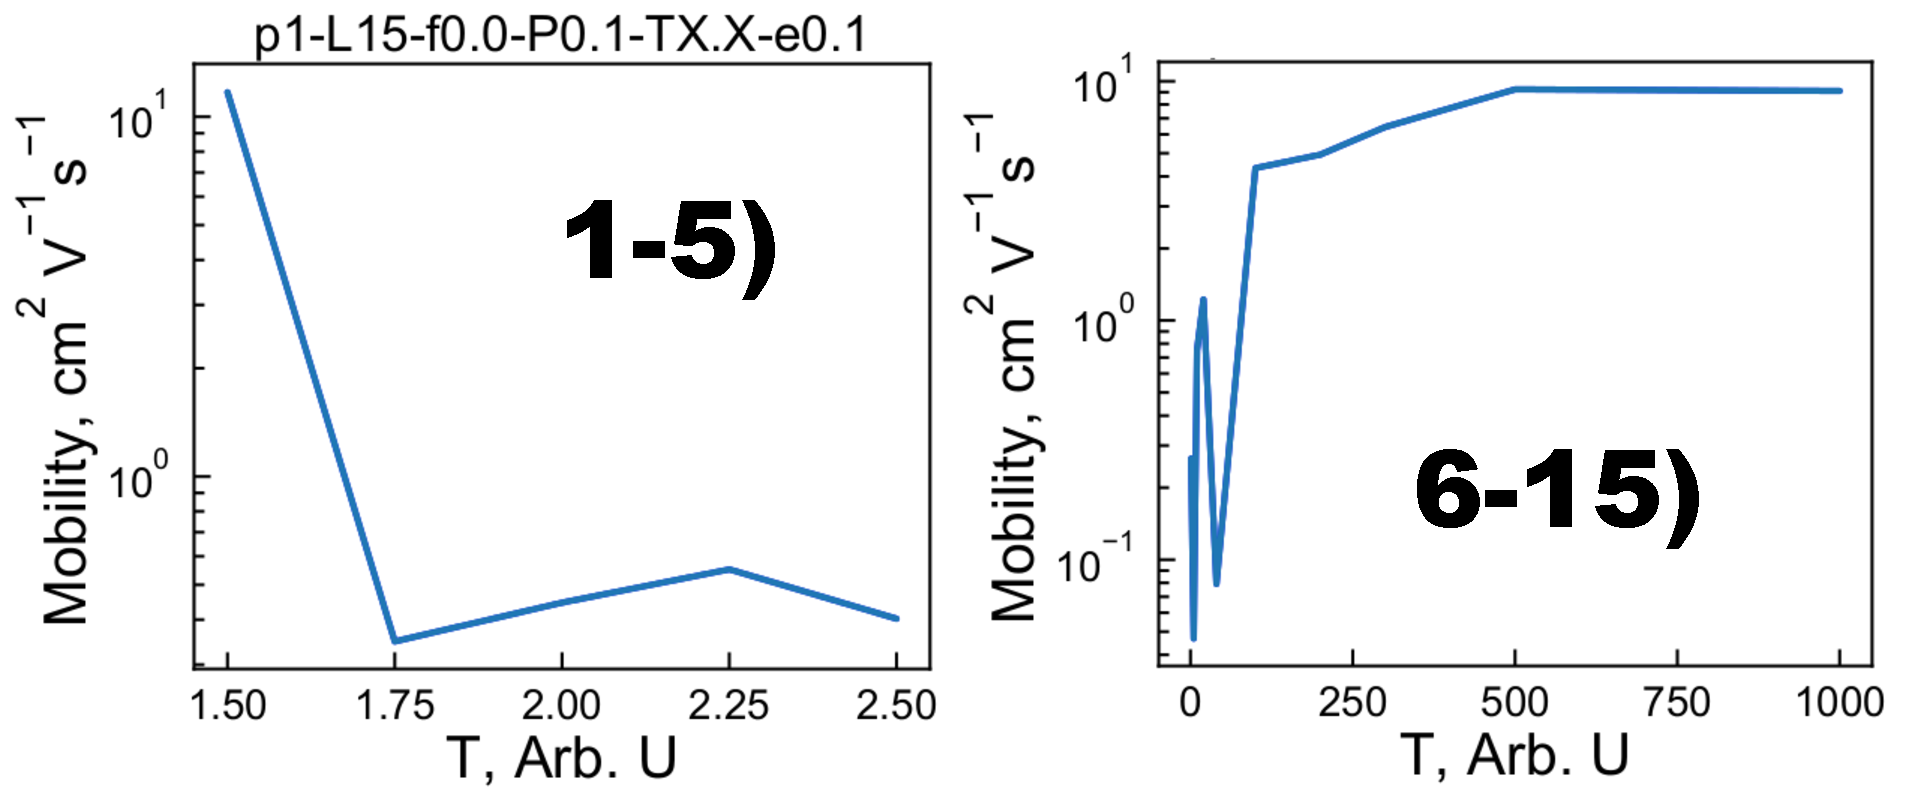
\includegraphics[width=\textwidth]{Figures/mobilityHole.pdf}
    \caption{The mobility trends observed over all jobs.}
	\label{fig:Mob}
\end{figure}

Representative Values From Literature:
\begin{itemize}
    \item{Density: \SI{1.10}{\gcm}\cite{Newbloom2012a}}
\item{Mobility: \SI{1E-5}{} - \SI{1E-3}{\mobunits}\cite{Ballantyne2008b,Mauer2010,Pandey2000,Kim2006}}
\end{itemize}

\clearpage

\subsection{3D Carrier Network}

\begin{figure}[h!]\centering
	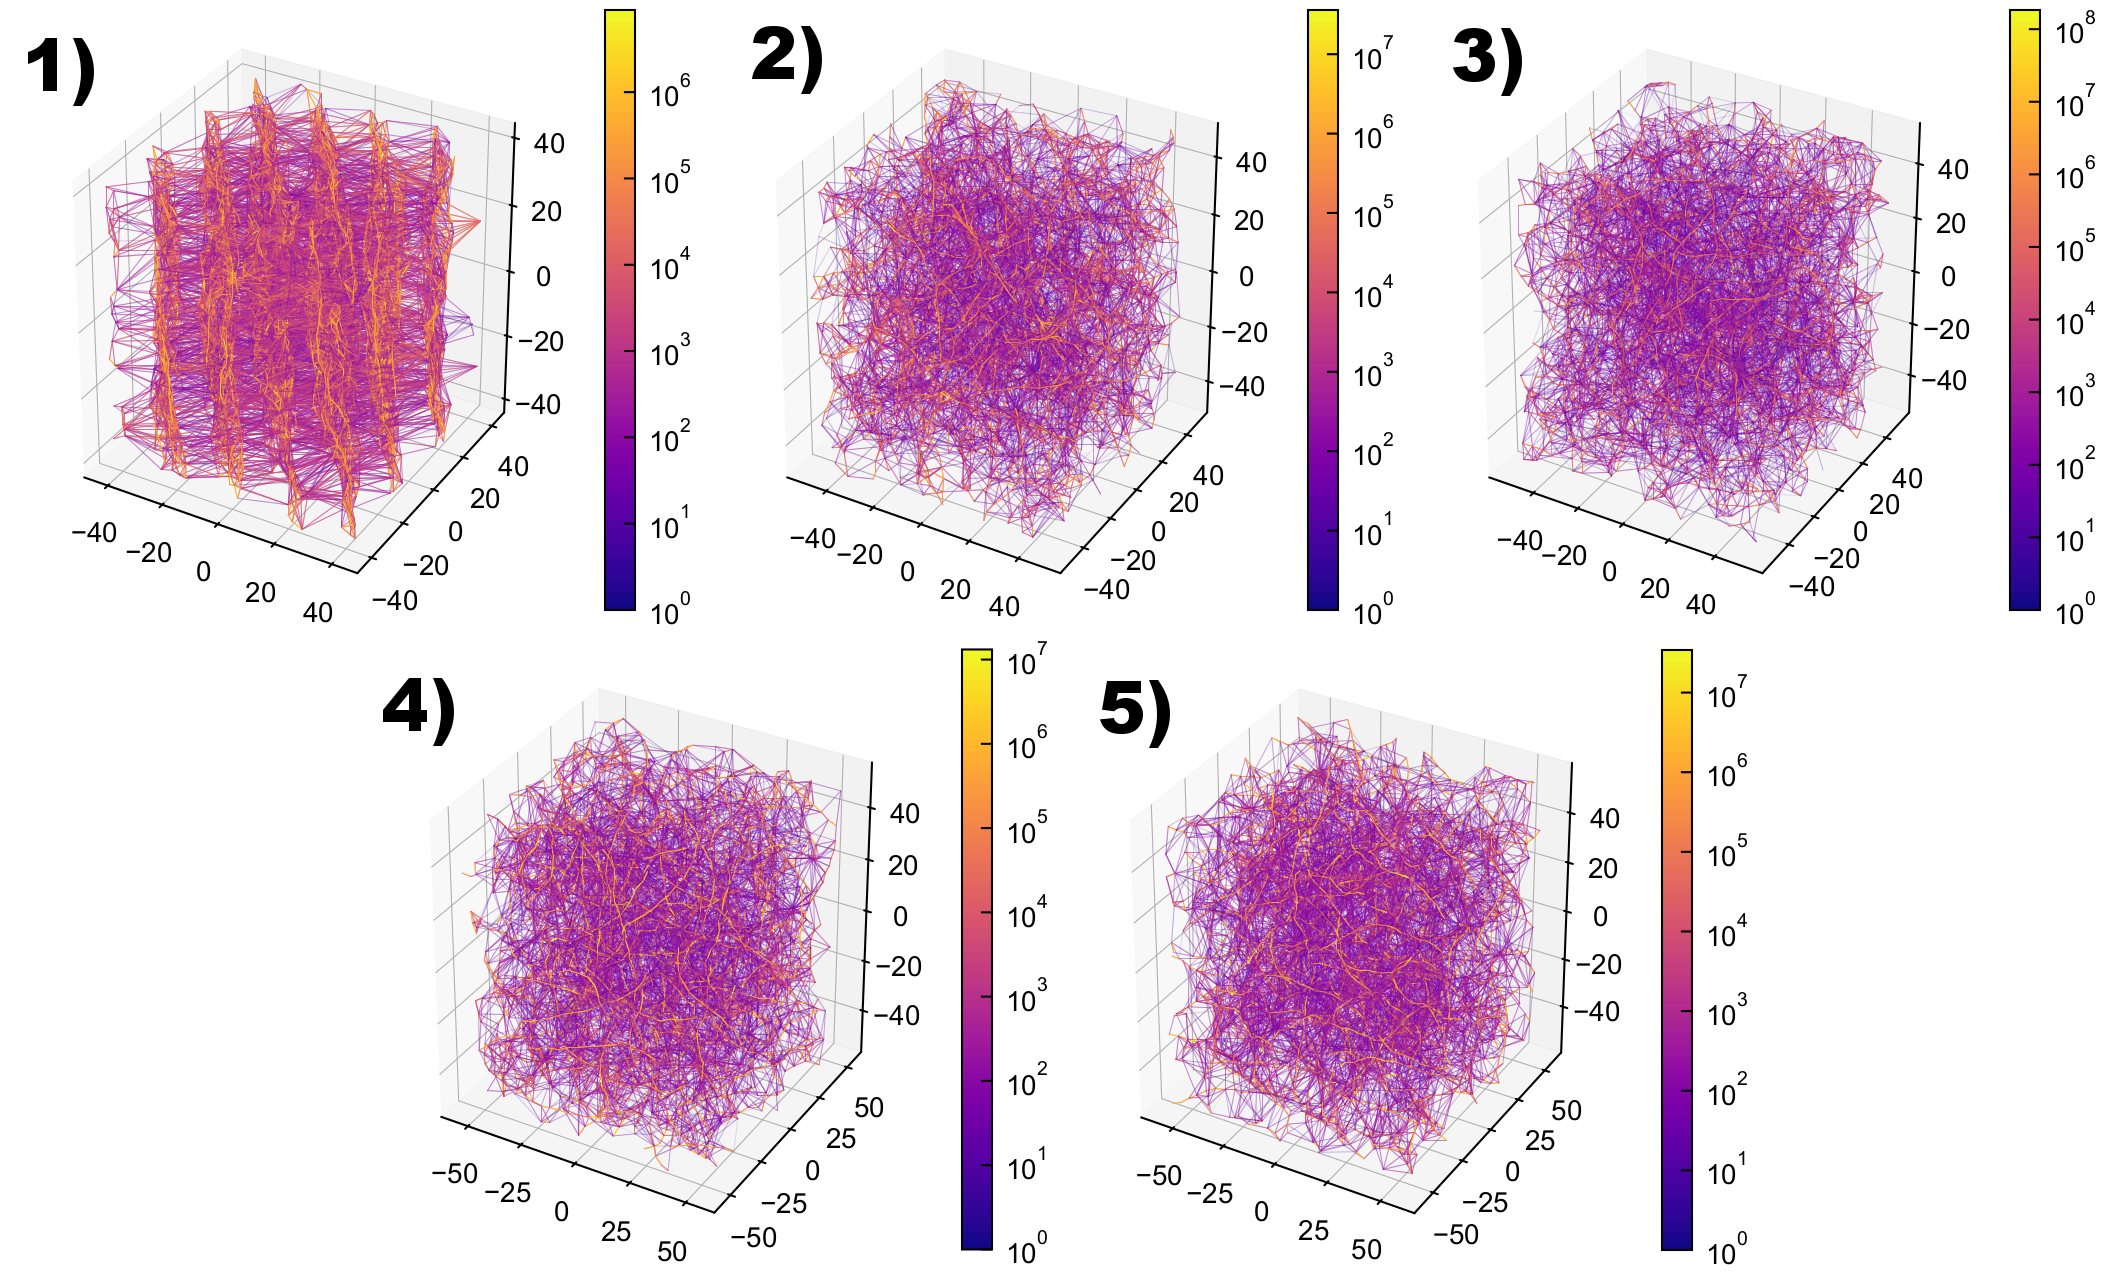
\includegraphics[width=\textwidth]{Figures/3dHole.png}
    \caption{The 3D heatmap of charge transport routes within the morphologies \textbf{1} - \textbf{5}.
    More yellow routes describe commonly accessed hops between pairs of chromophores, whereas more purple routes are less widely used in the KMC simulations.
    Each node therefore represents the location of a single chromophore.
The intensity value for the route is currently taken to be \texttt{I $=$ np.log10(freq) $/$ np.log10(max\_freq)}.}
	\label{fig:3dNetwork}
\end{figure}


\begin{figure}[h!]\centering
	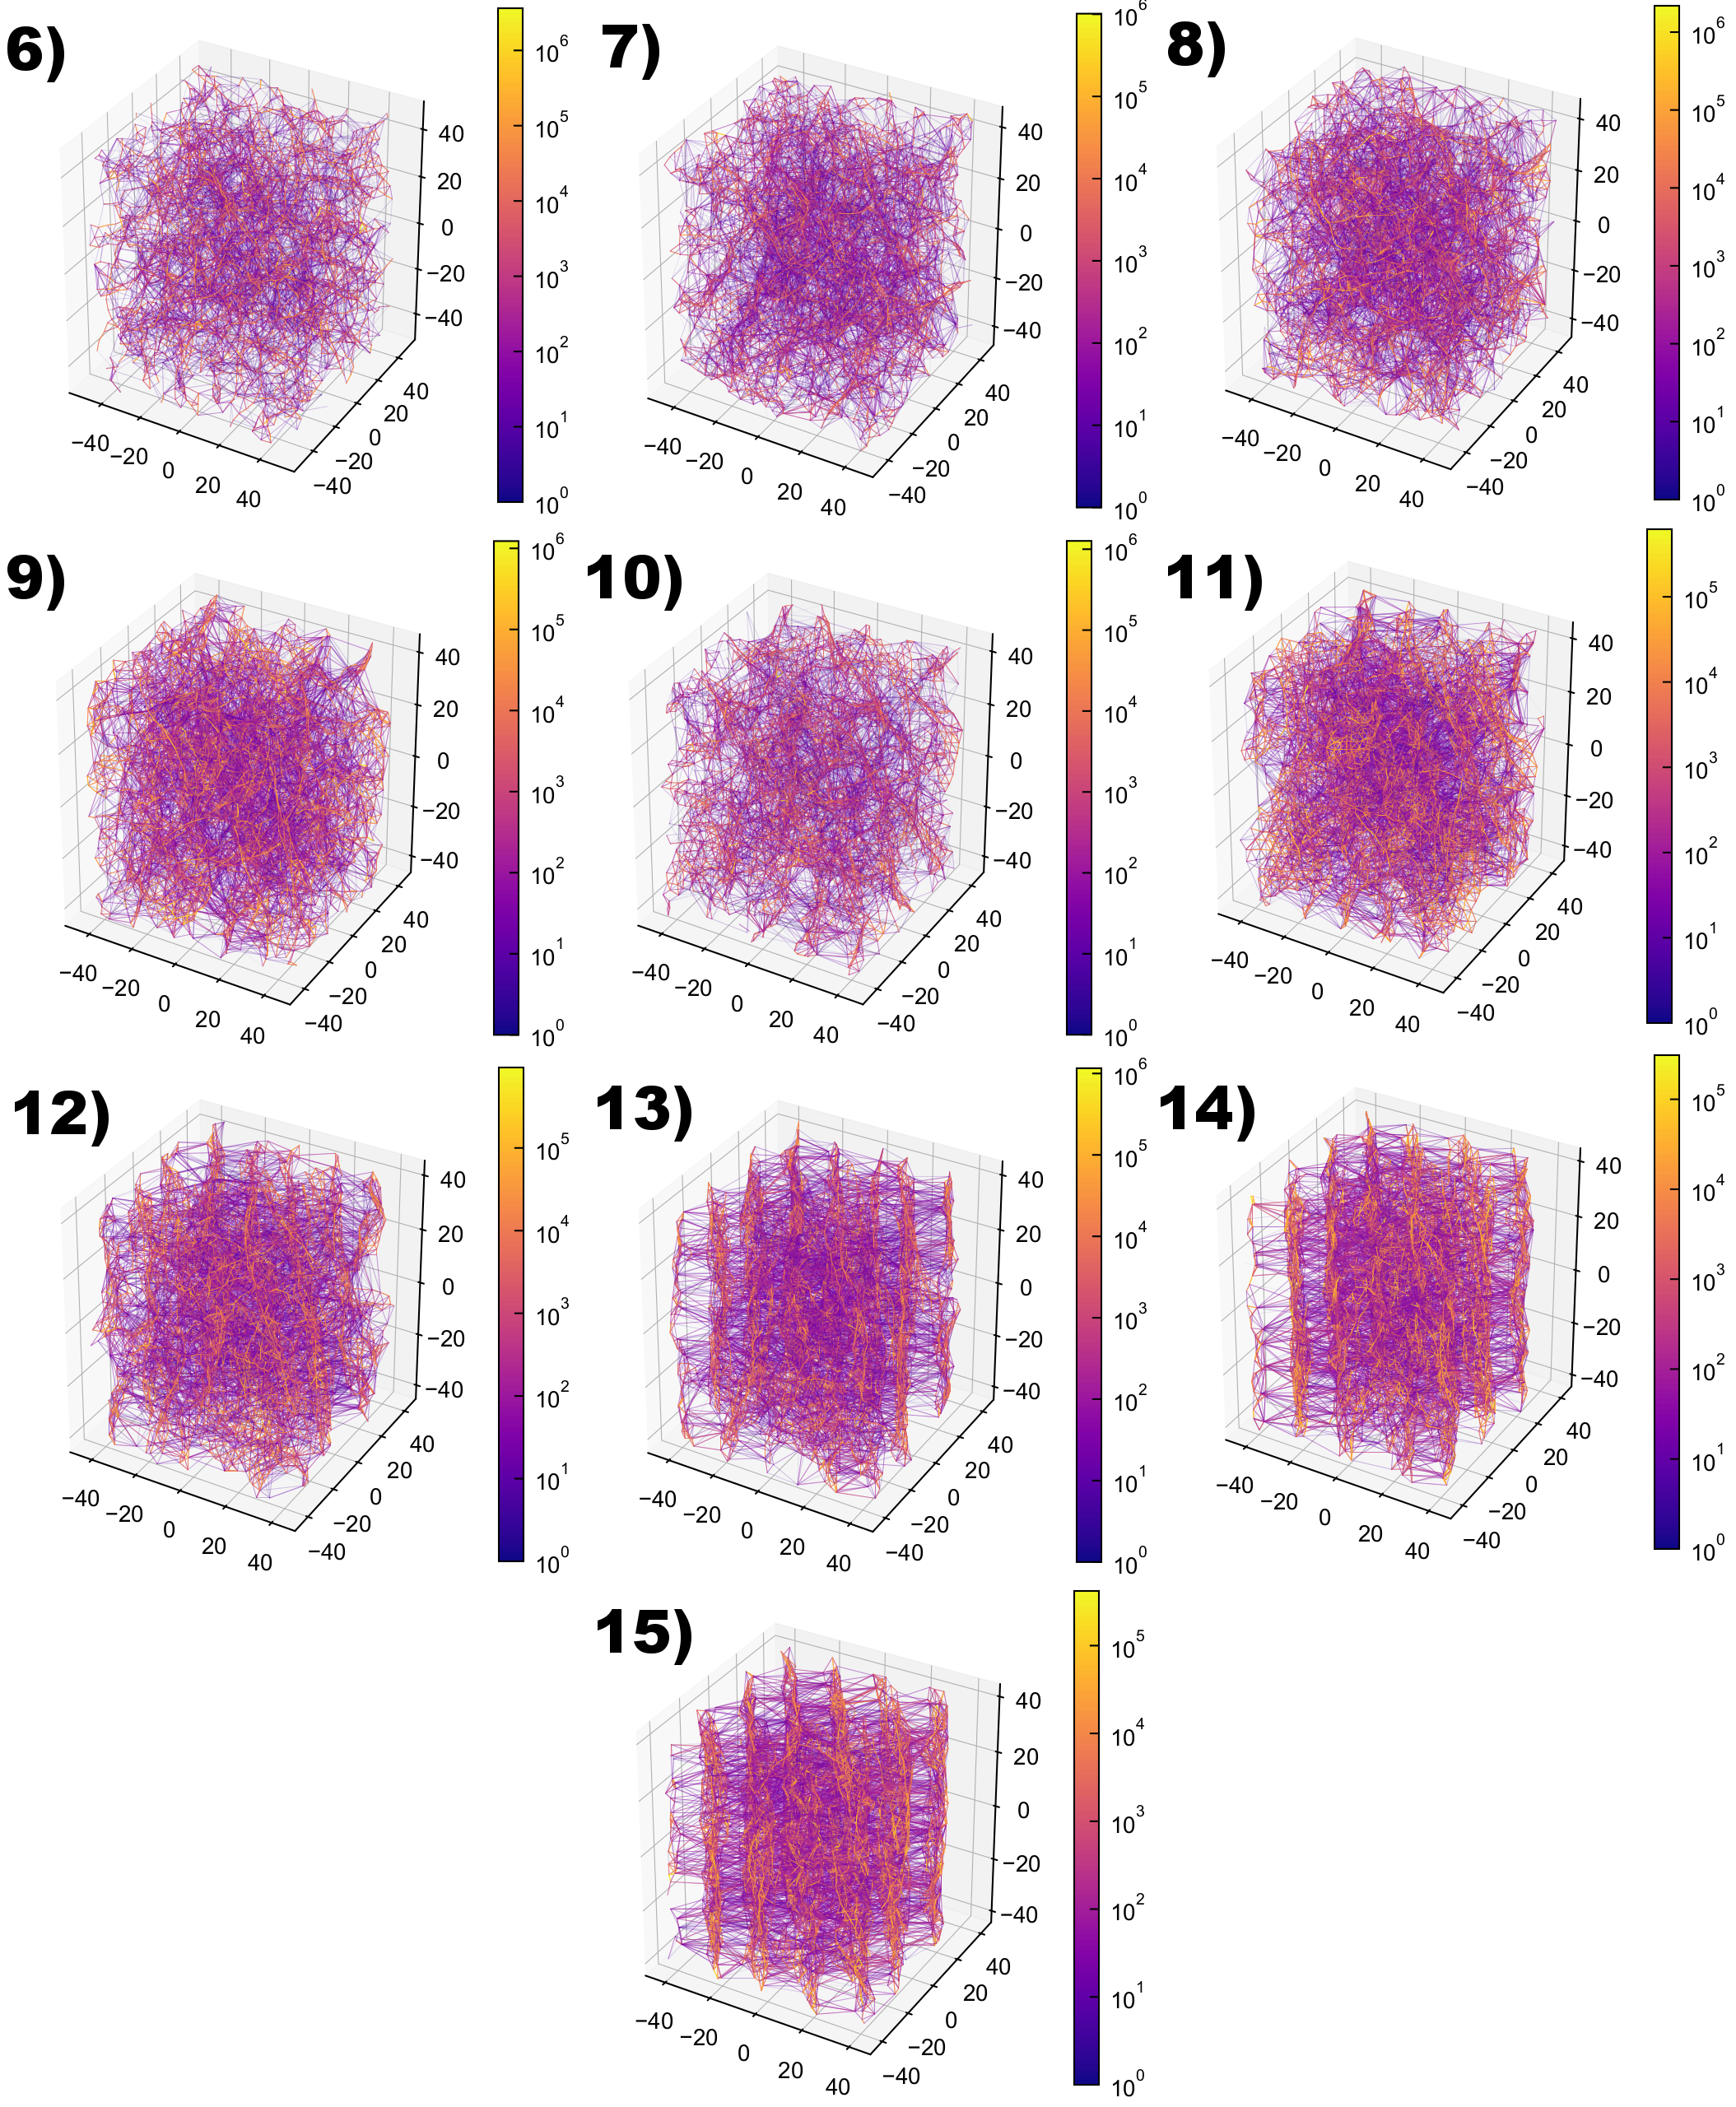
\includegraphics[width=\textwidth]{Figures/3dHoleFrame.png}
    \caption{The 3D heatmap of charge transport routes within the morphologies \textbf{6} - \textbf{15}.
    More yellow routes describe commonly accessed hops between pairs of chromophores, whereas more purple routes are less widely used in the KMC simulations.
    Each node therefore represents the location of a single chromophore.
The intensity value for the route is currently taken to be \texttt{I $=$ np.log10(freq) $/$ np.log10(max\_freq)}.}
	\label{fig:3dNetworkFrame}
\end{figure}


\begin{figure}[h!]\centering
	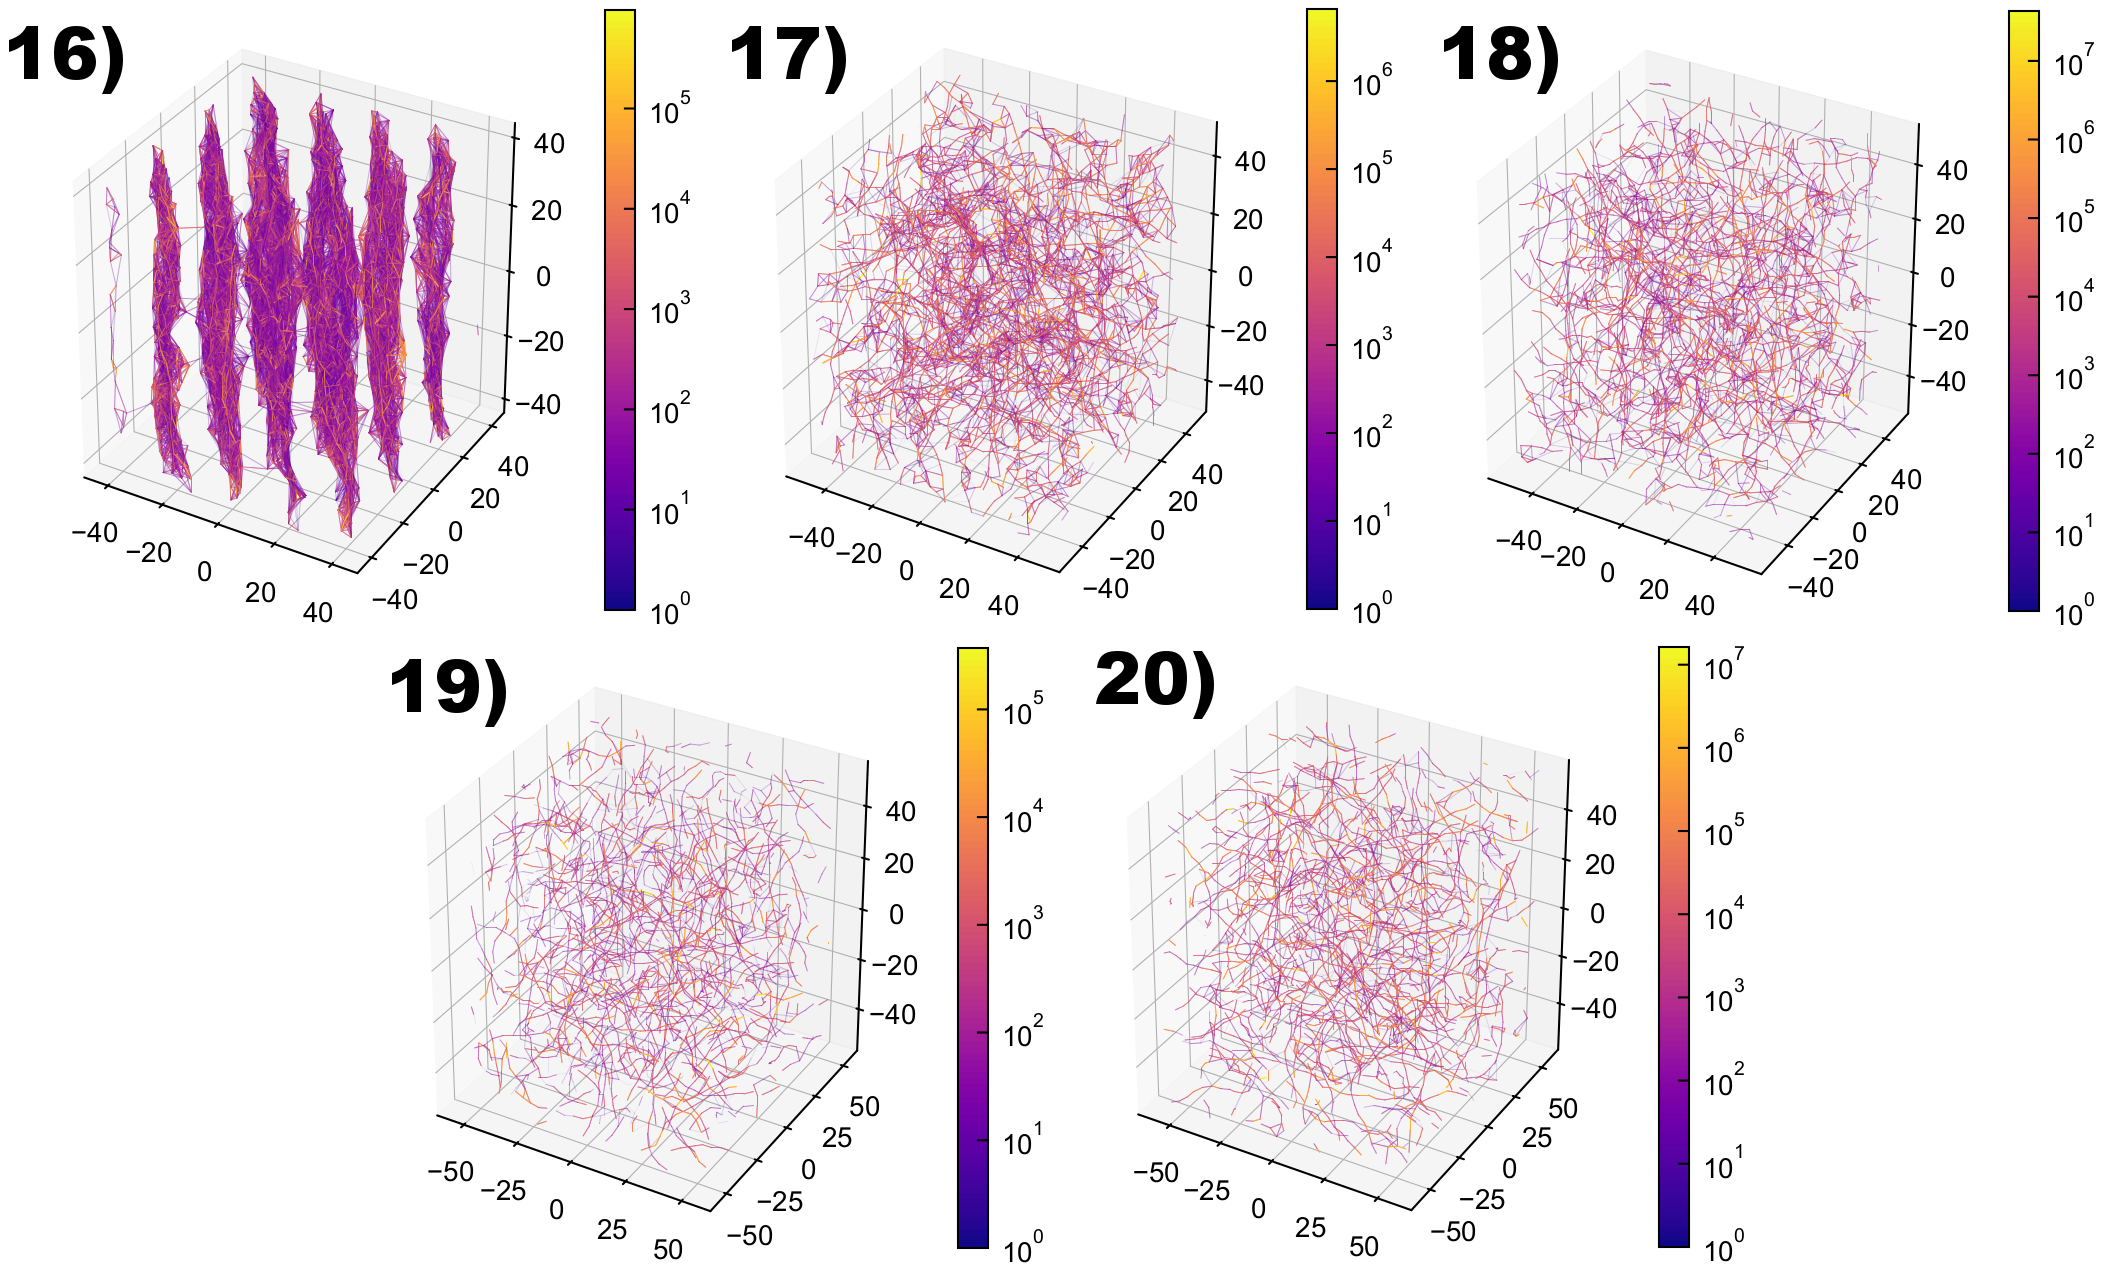
\includegraphics[width=\textwidth]{Figures/3dHoleOrig.png}
    \caption{The 3D heatmap of charge transport routes within the morphologies \textbf{16} - \textbf{20}.
    More yellow routes describe commonly accessed hops between pairs of chromophores, whereas more purple routes are less widely used in the KMC simulations.
    Each node therefore represents the location of a single chromophore.
The intensity value for the route is currently taken to be \texttt{I $=$ np.log10(freq) $/$ np.log10(max\_freq)}.}
	\label{fig:3dNetworkOrig}
\end{figure}


\begin{figure}[h!]\centering
	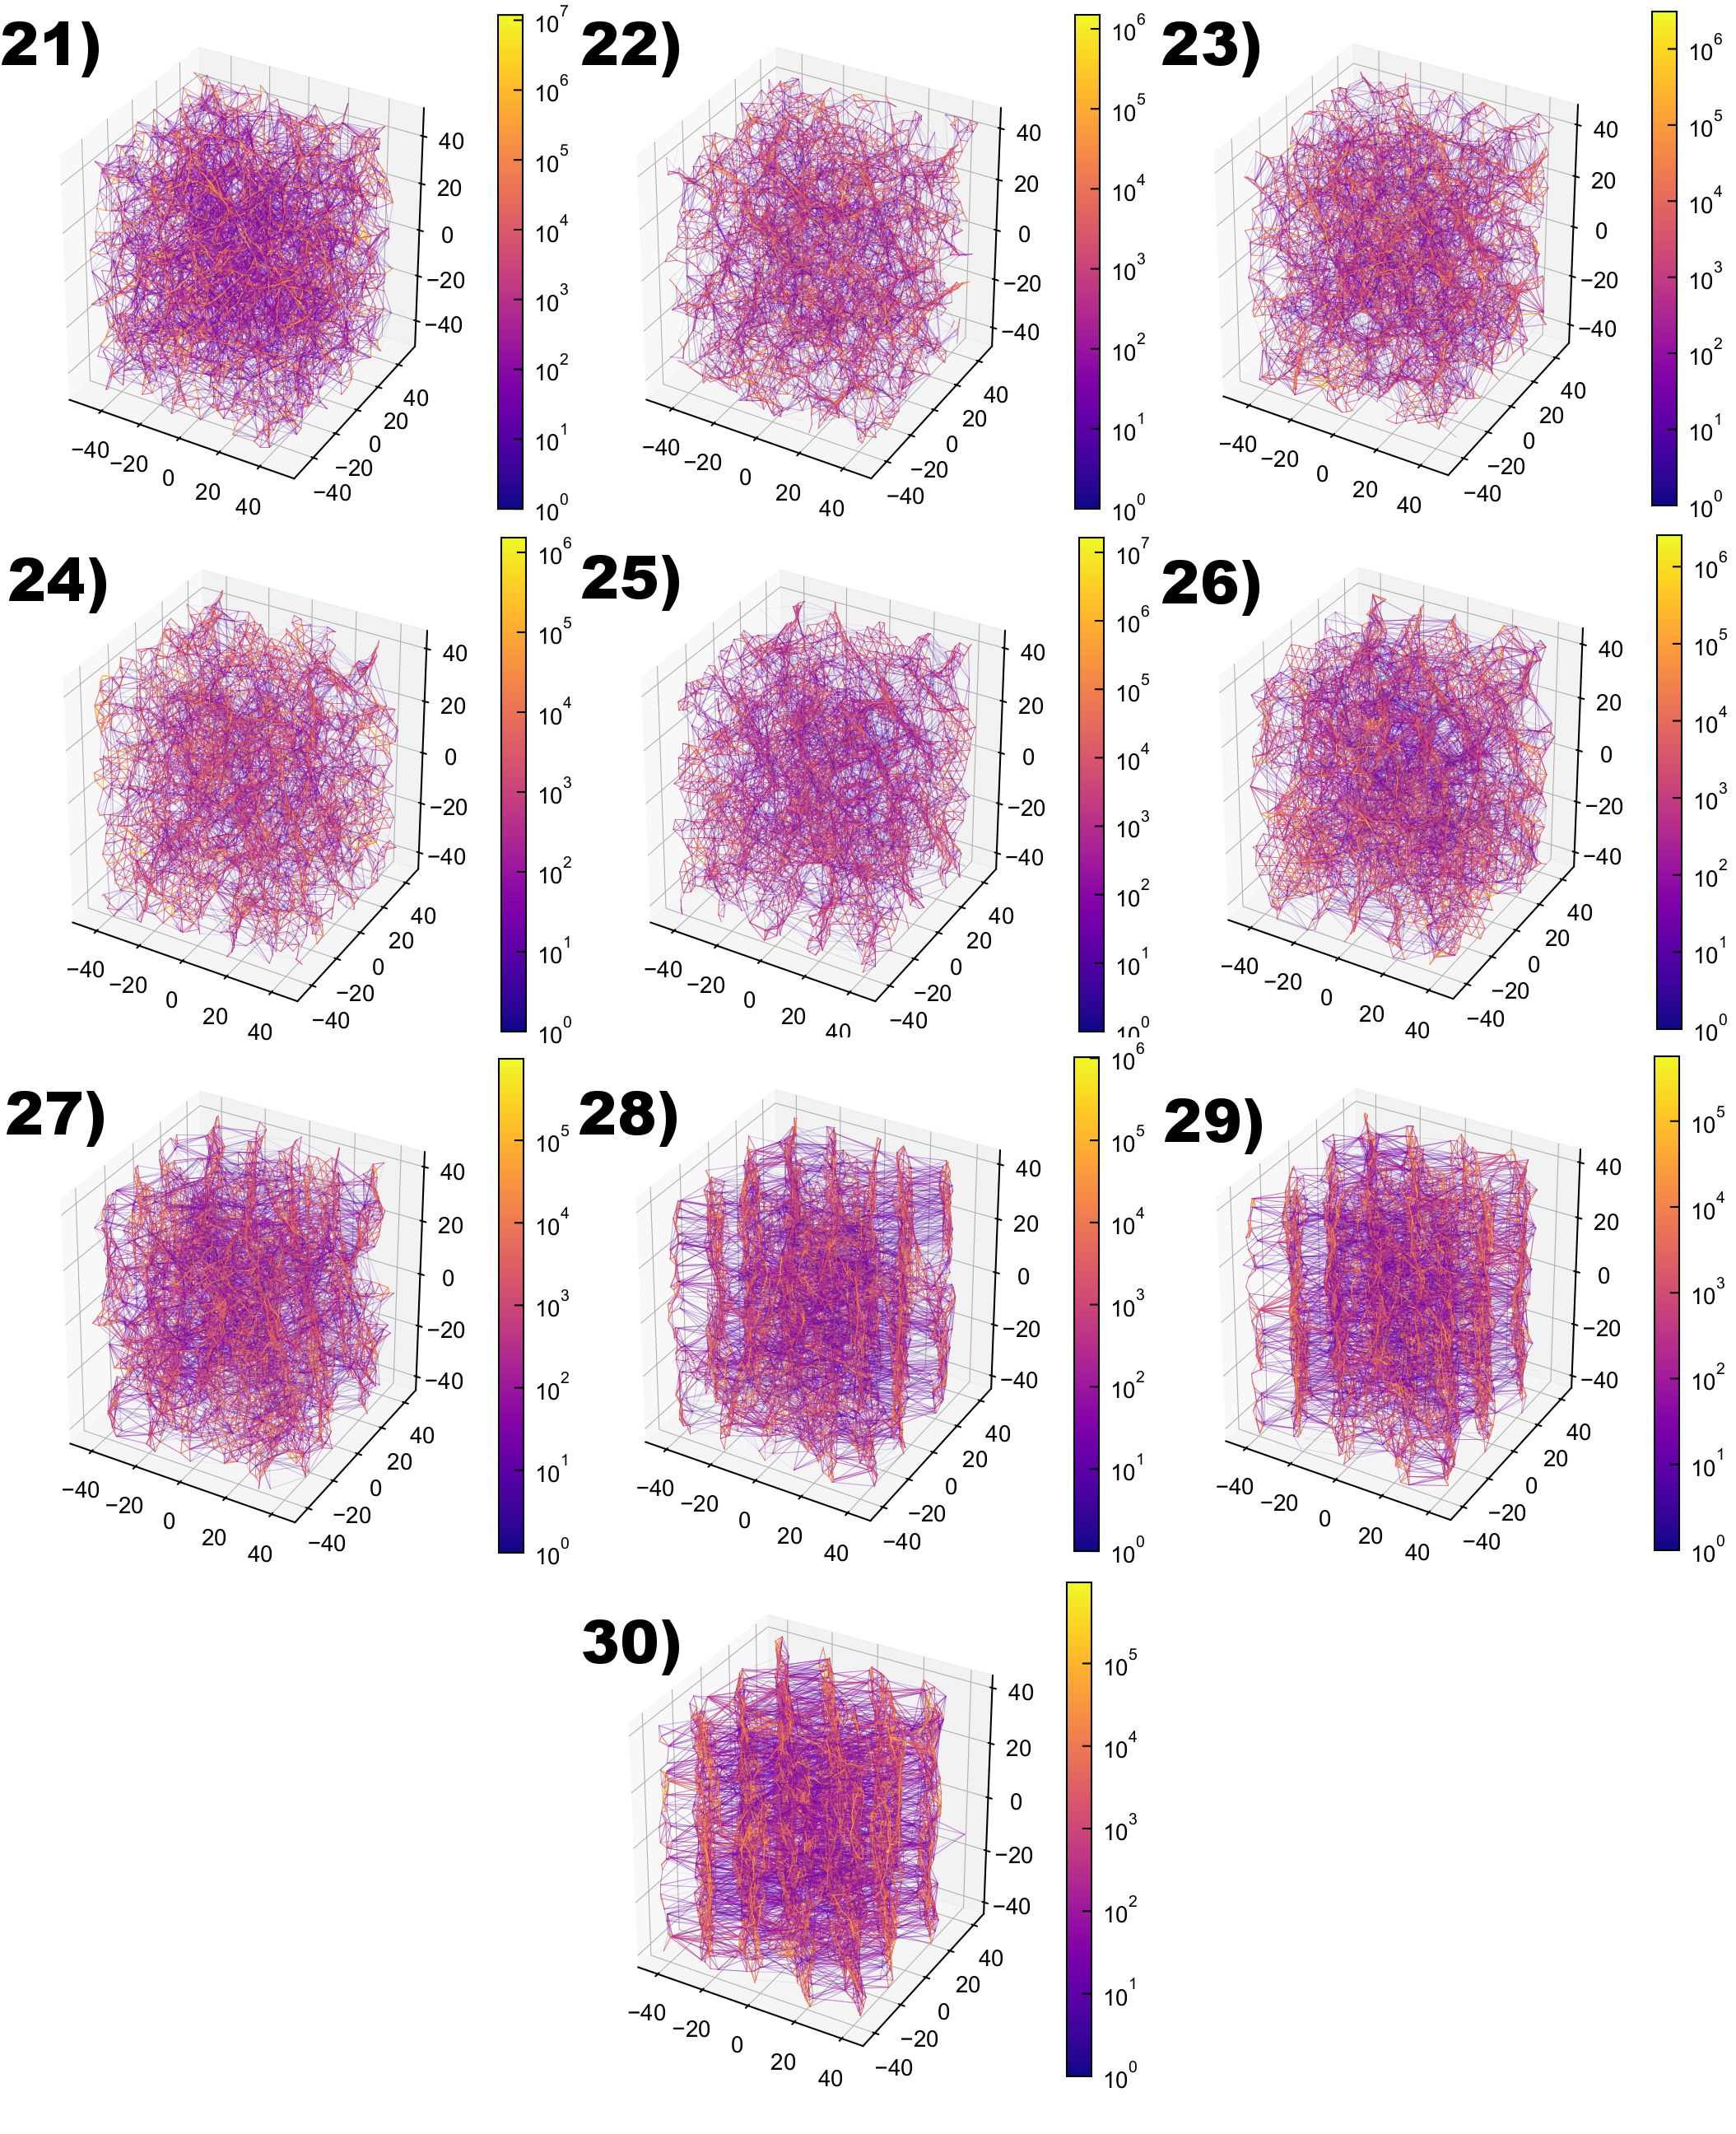
\includegraphics[width=\textwidth]{Figures/3dHoleFrameOrig.png}
    \caption{The 3D heatmap of charge transport routes within the morphologies \textbf{21} - \textbf{30}.
    More yellow routes describe commonly accessed hops between pairs of chromophores, whereas more purple routes are less widely used in the KMC simulations.
    Each node therefore represents the location of a single chromophore.
The intensity value for the route is currently taken to be \texttt{I $=$ np.log10(freq) $/$ np.log10(max\_freq)}.}
	\label{fig:3dNetworkFrameOrig}
\end{figure}

\clearpage
\subsection{Anisotropies}


\begin{figure}[h!]\centering
	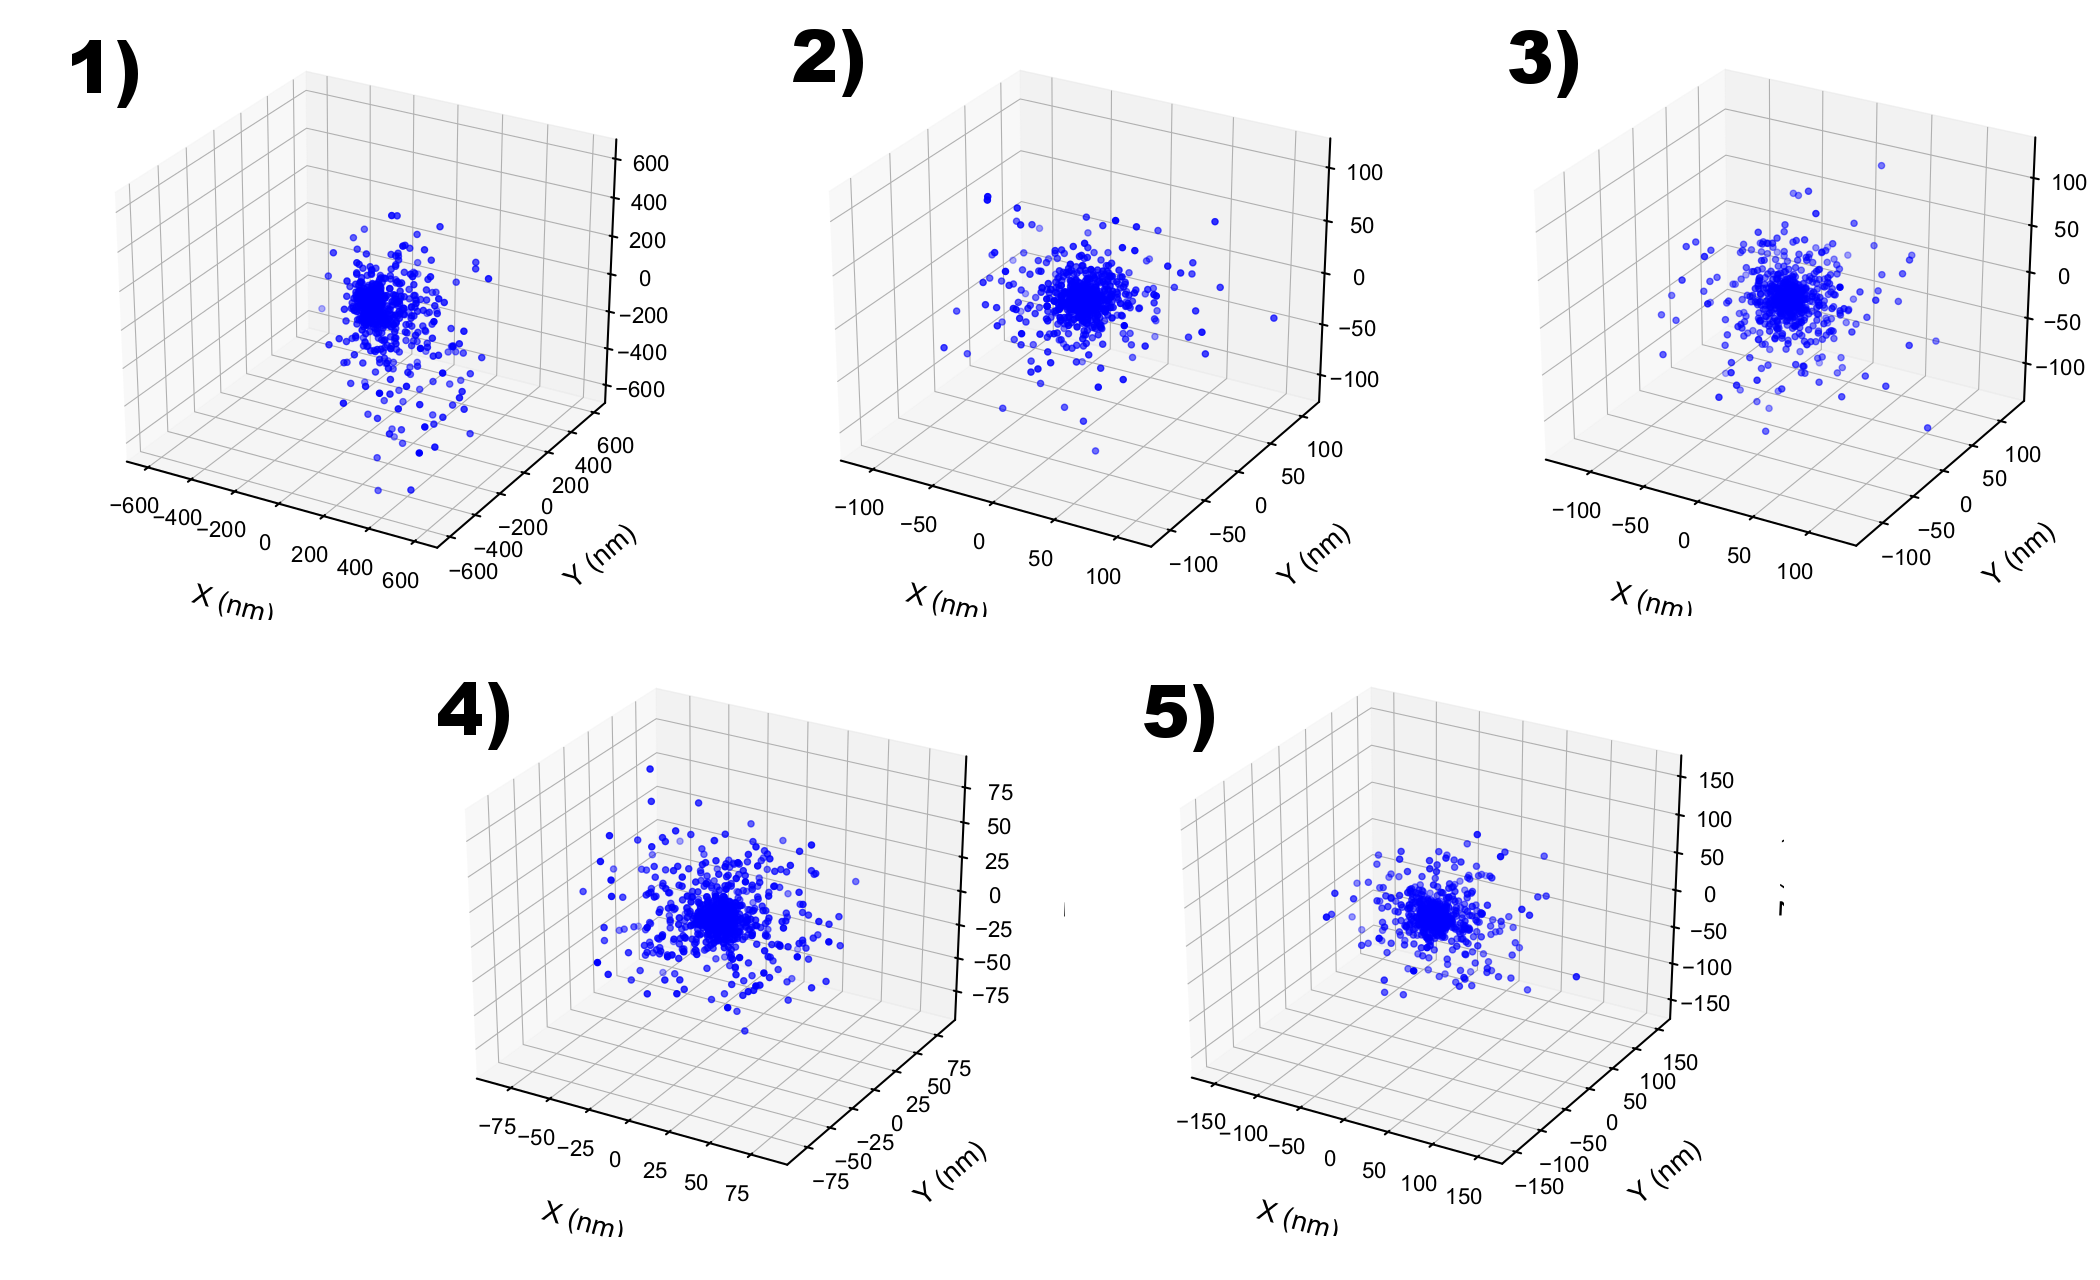
\includegraphics[width=\textwidth]{Figures/anisotropyHole.png}
    \caption{The periodic anisotropies of the carrier transport within the morphologies \textbf{1} - \textbf{5}.}
	\label{fig:Anis}
\end{figure}

\begin{figure}[h!]\centering
	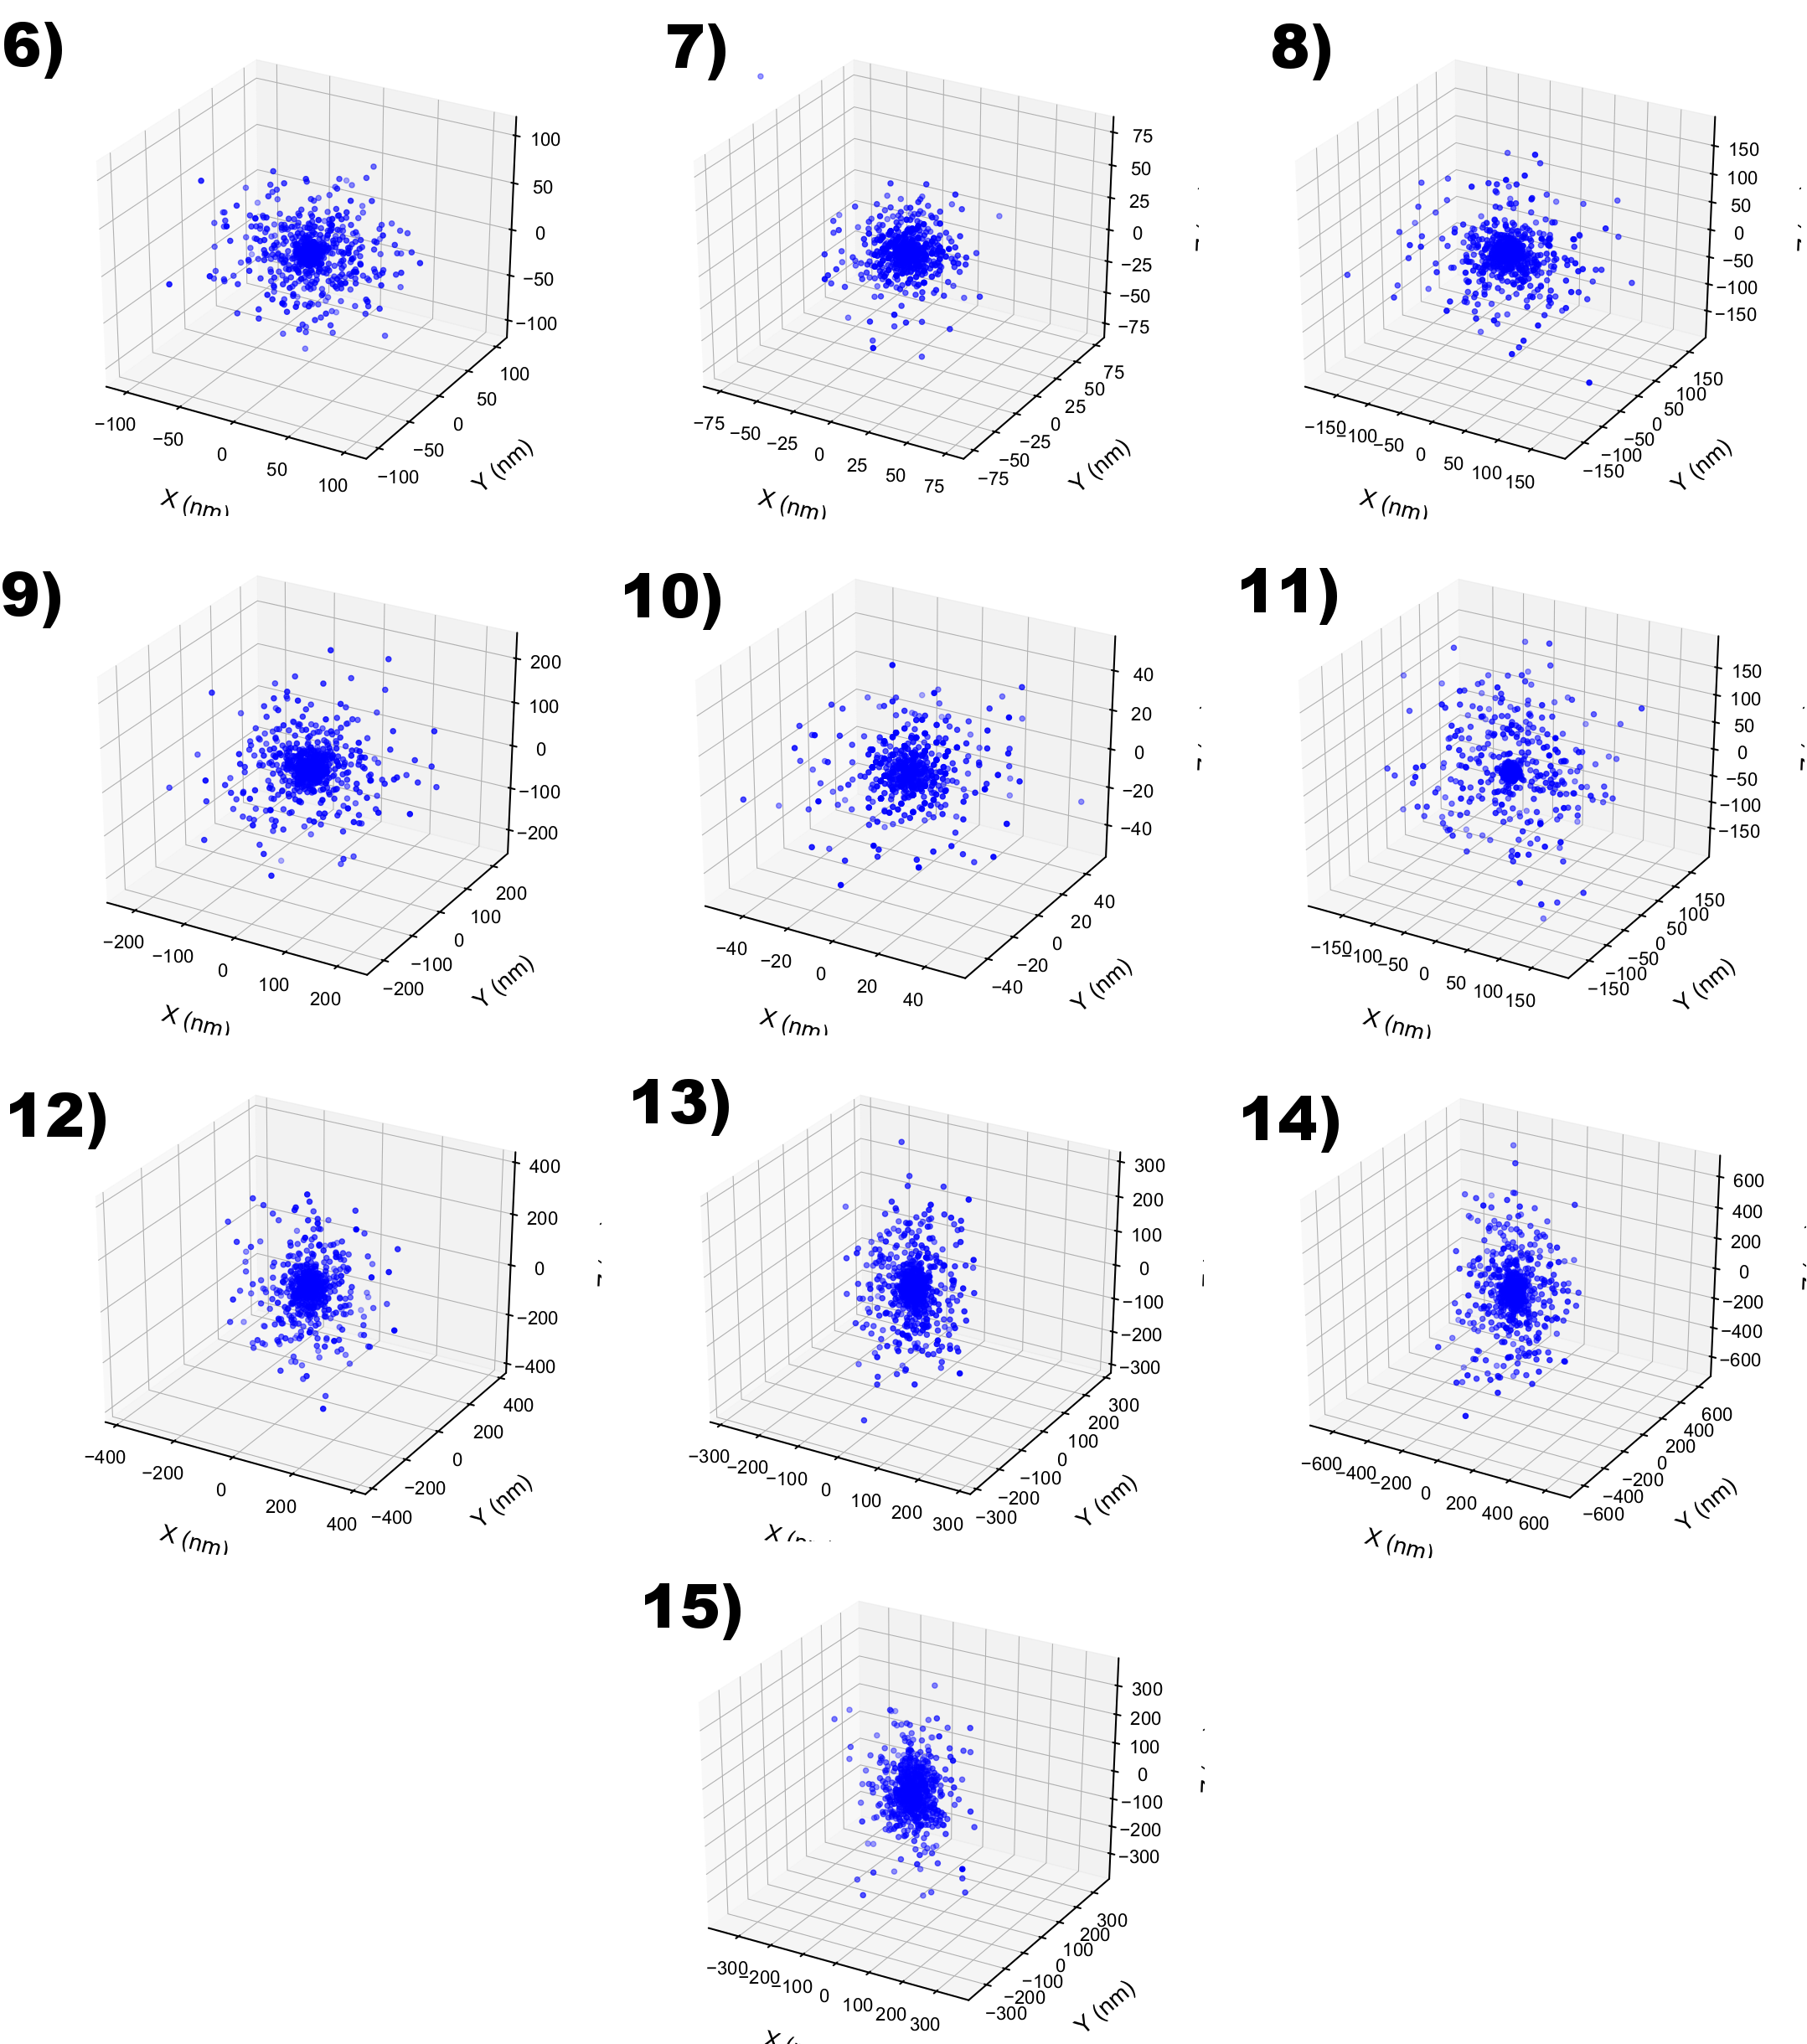
\includegraphics[width=\textwidth]{Figures/anisotropyHoleFrame.png}
    \caption{The periodic anisotropies of the carrier transport within the morphologies \textbf{6} - \textbf{15}.}
	\label{fig:AnisFrame}
\end{figure}


\begin{figure}[h!]\centering
	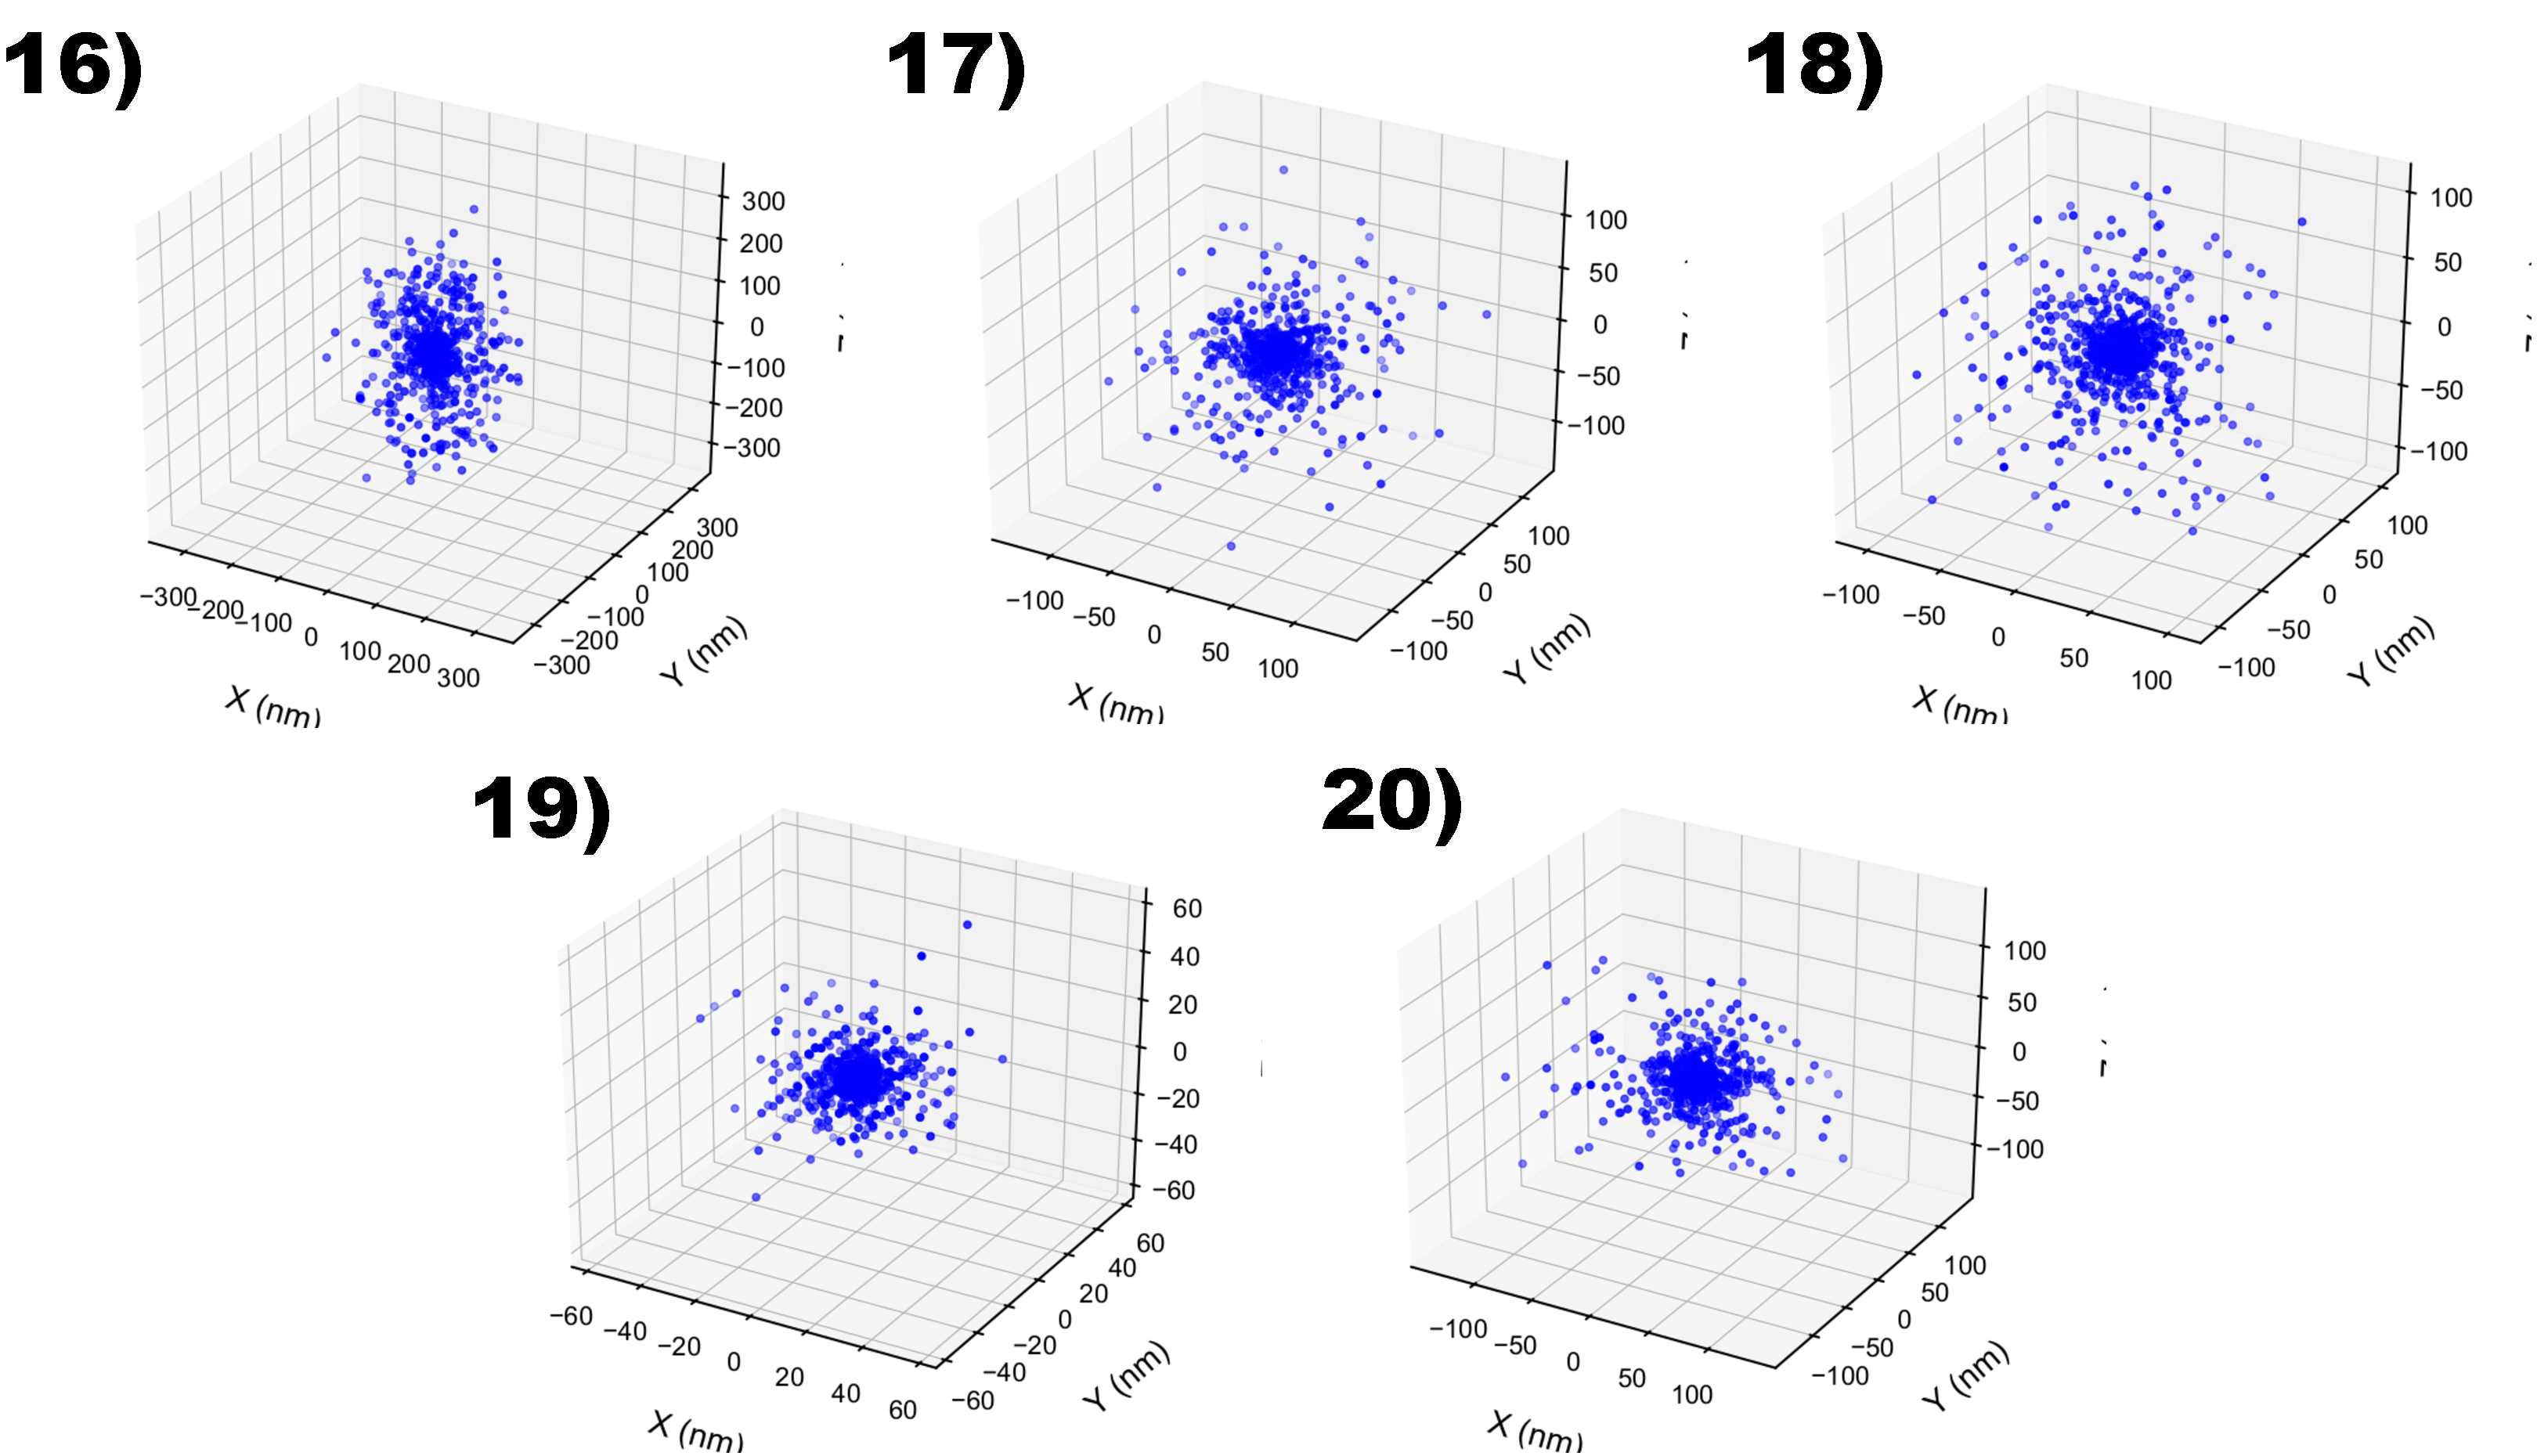
\includegraphics[width=\textwidth]{Figures/anisotropyHoleOrig.pdf}
    \caption{The periodic anisotropies of the carrier transport within the morphologies \textbf{16} - \textbf{20}.}
	\label{fig:AnisOrig}
\end{figure}

\begin{figure}[h!]\centering
	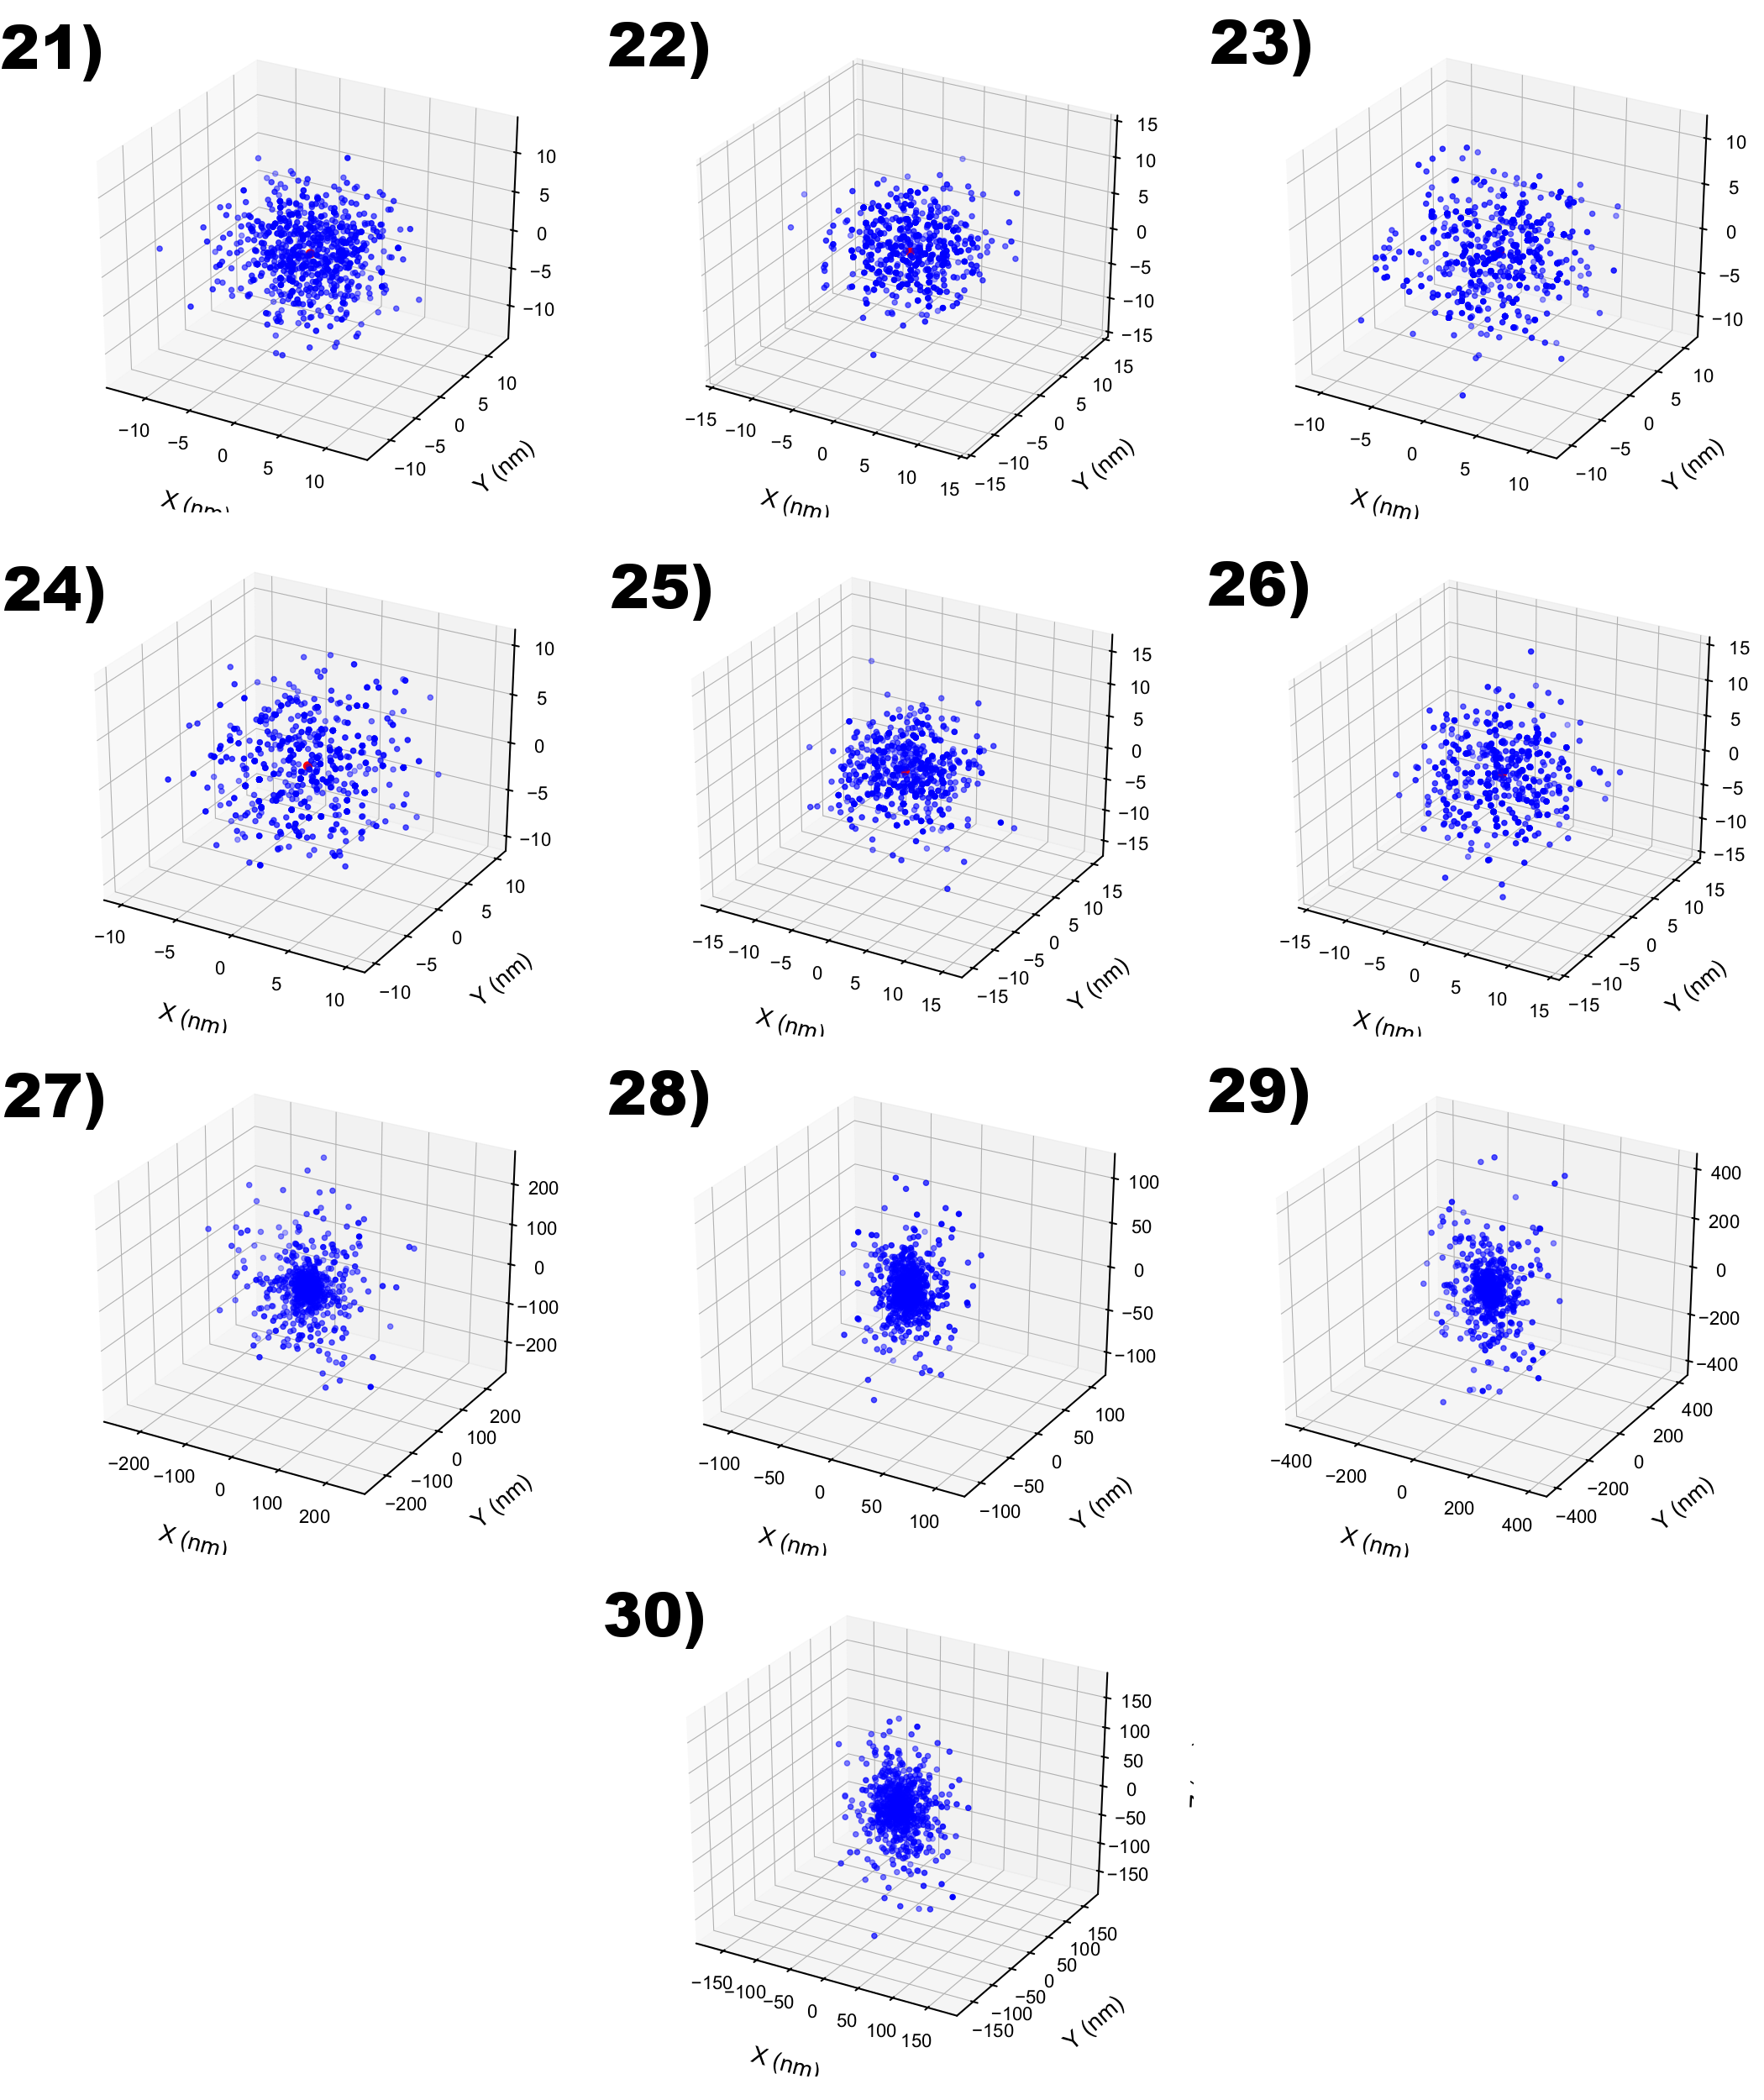
\includegraphics[width=\textwidth]{Figures/anisotropyHoleFrameOrig.png}
    \caption{The periodic anisotropies of the carrier transport within the morphologies \textbf{21} - \textbf{30}.}
	\label{fig:AnisFrameOrig}
\end{figure}

\clearpage
\subsection{MSDs}


\begin{figure}[h!]\centering
	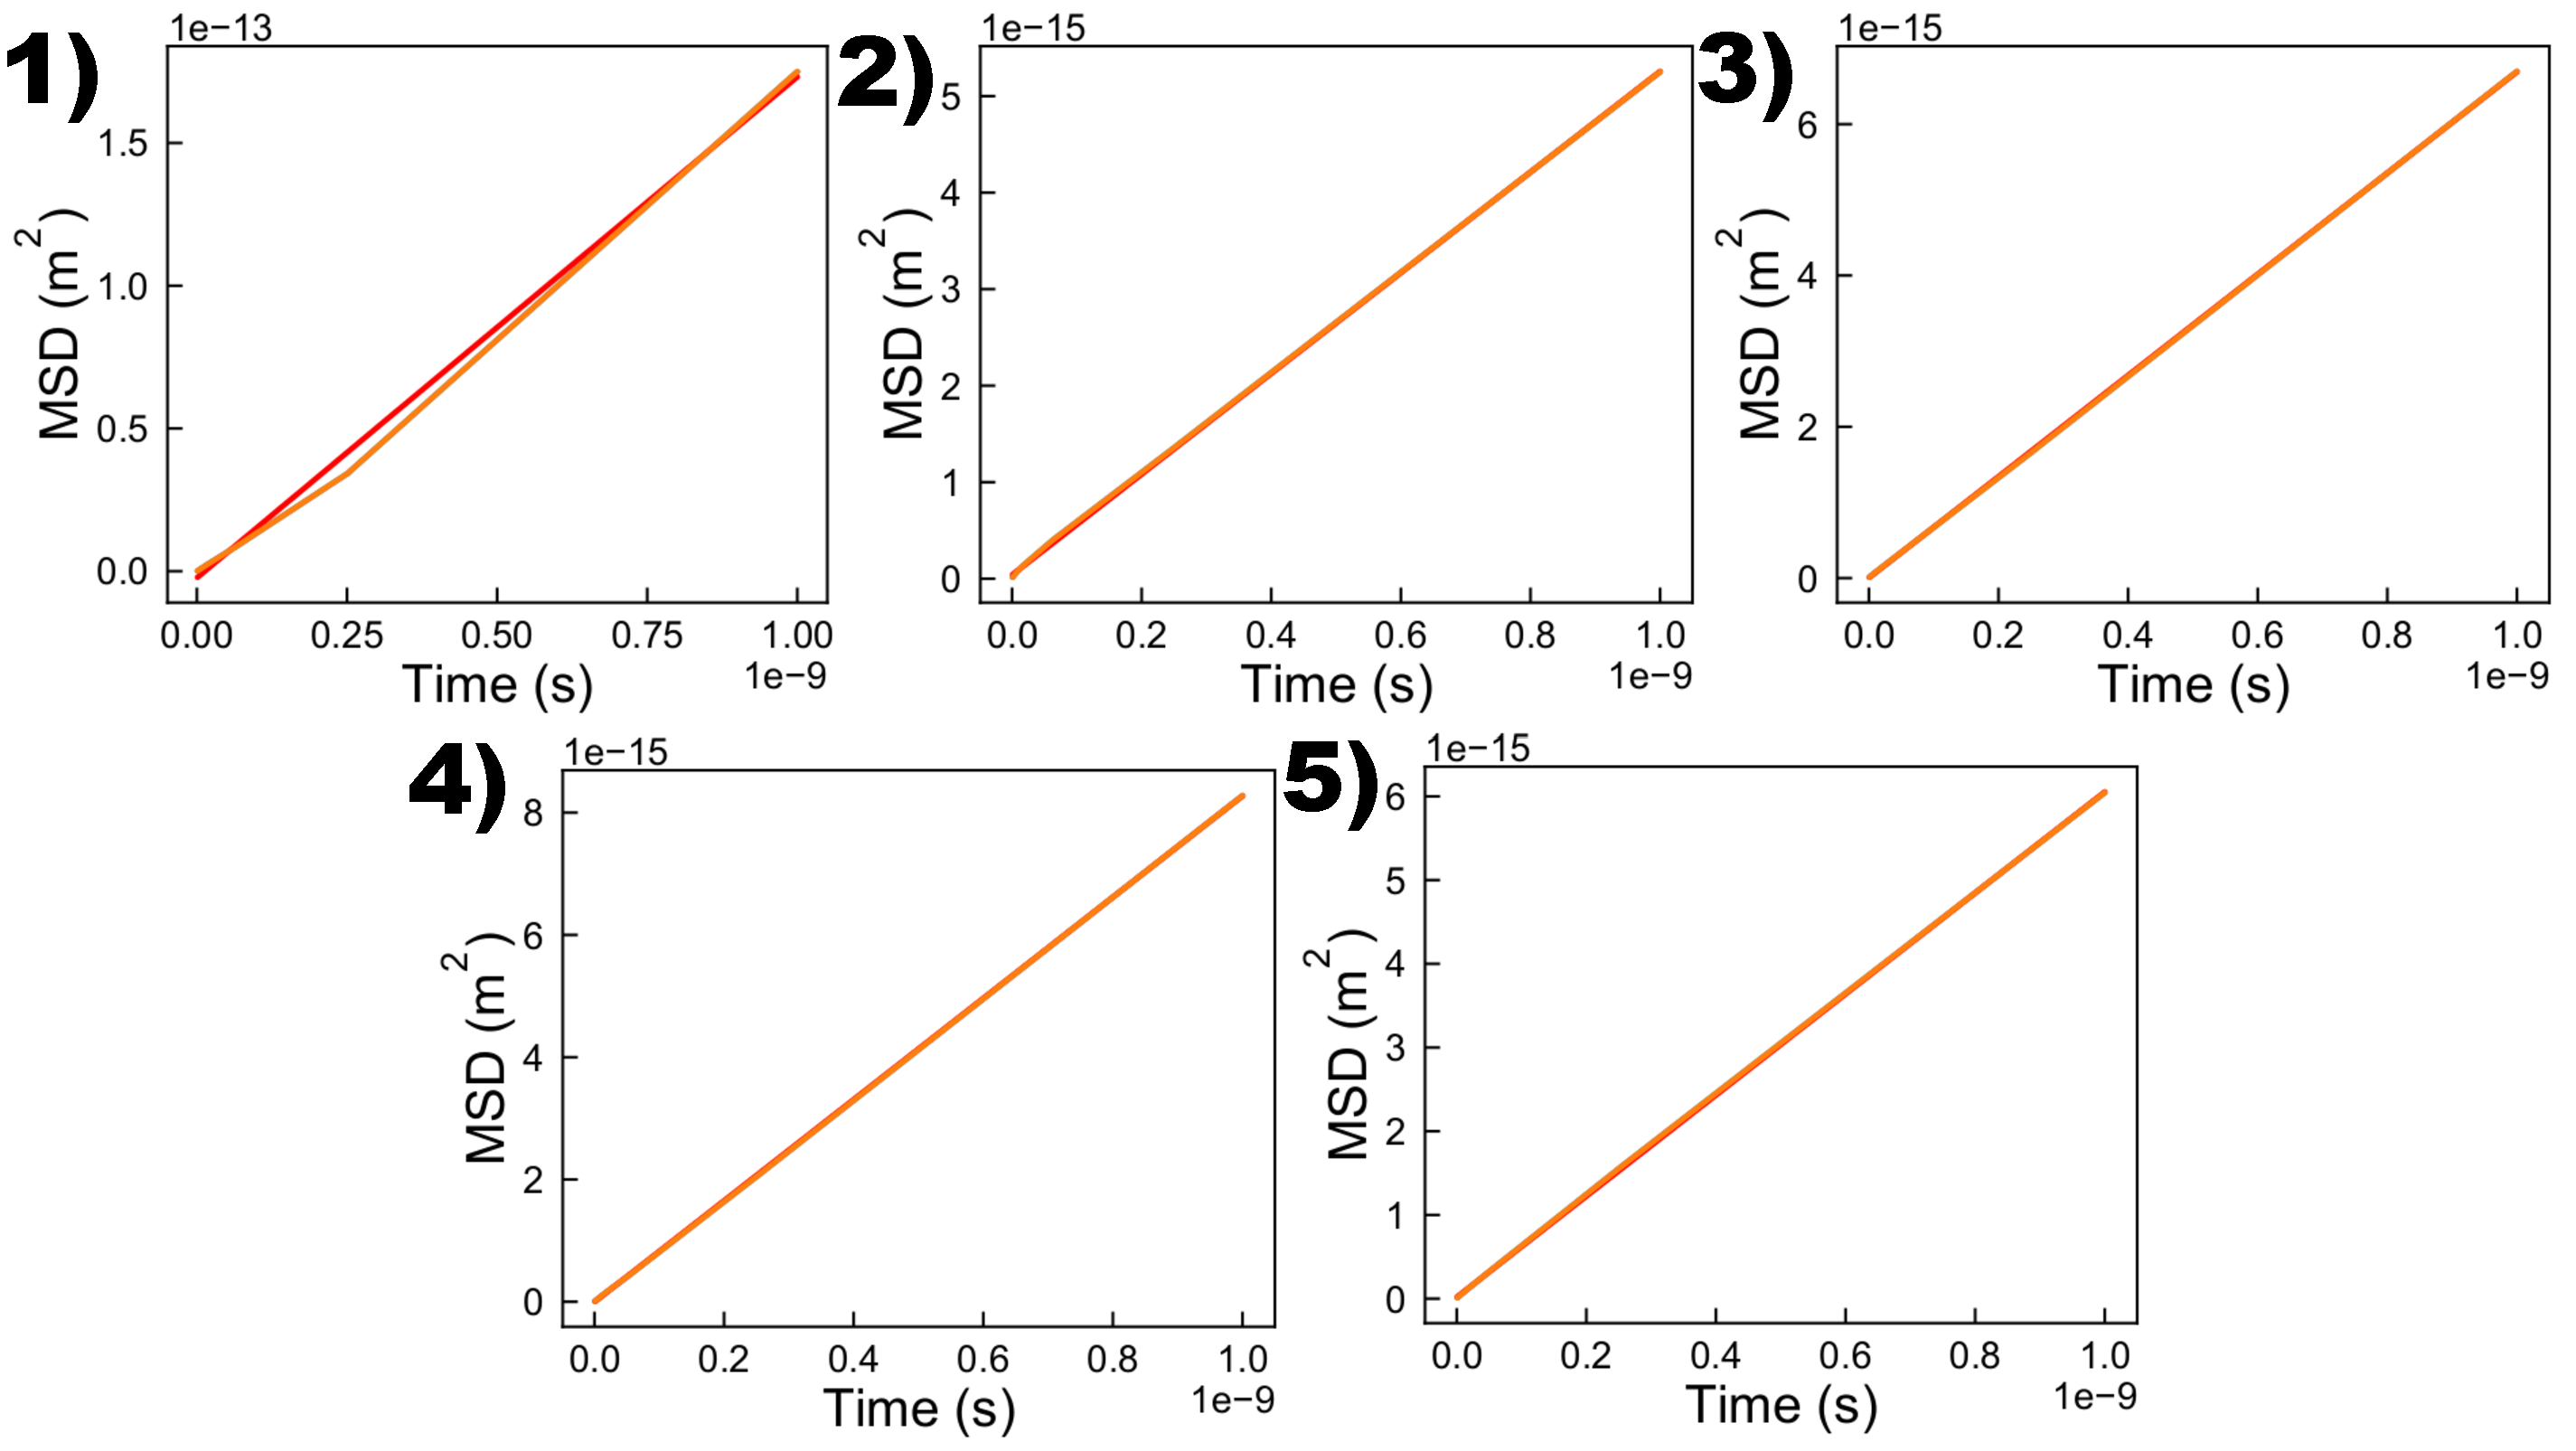
\includegraphics[width=\textwidth]{Figures/LinMSDHole.pdf}
    \caption{The linear mean squared displacement curves of the carriers within the morphologies \textbf{1} - \textbf{5}.}
	\label{fig:MSD}
\end{figure}


\begin{figure}[h!]\centering
	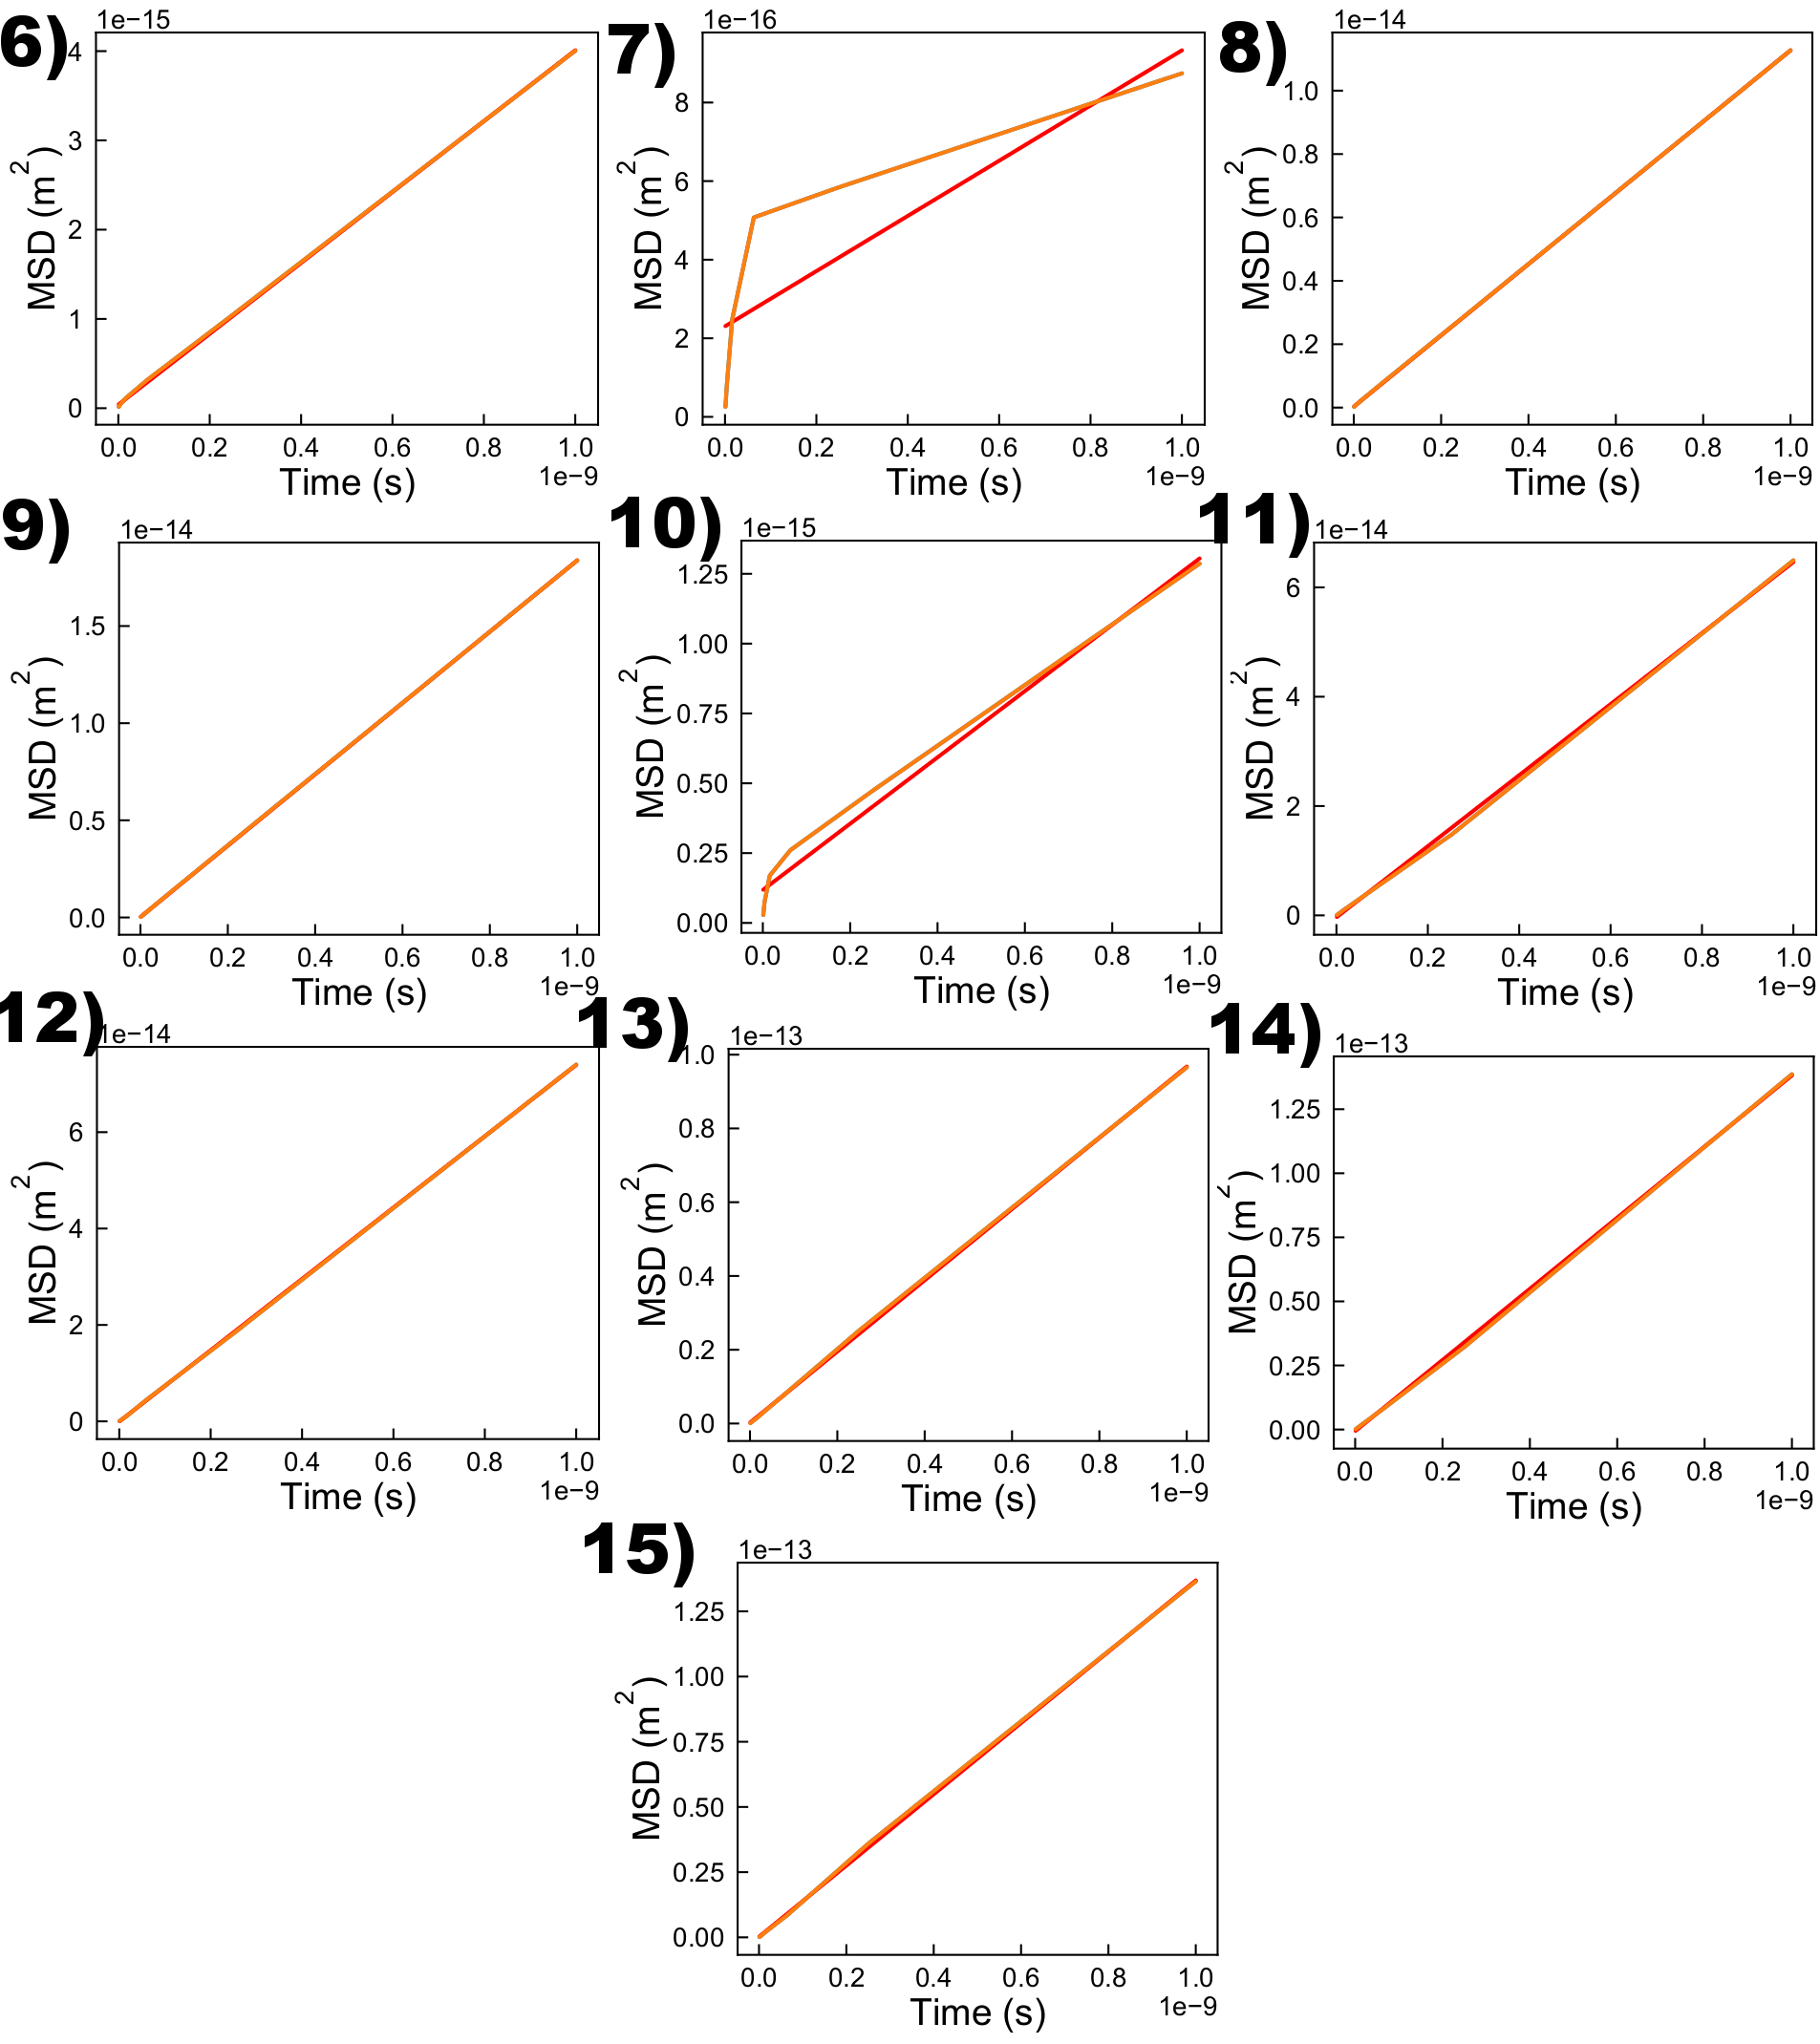
\includegraphics[width=\textwidth]{Figures/LinMSDHoleFrame.png}
    \caption{The linear mean squared displacement curves of the carriers within the morphologies \textbf{6} - \textbf{15}.}
	\label{fig:MSDFrame}
\end{figure}

\begin{figure}[h!]\centering
	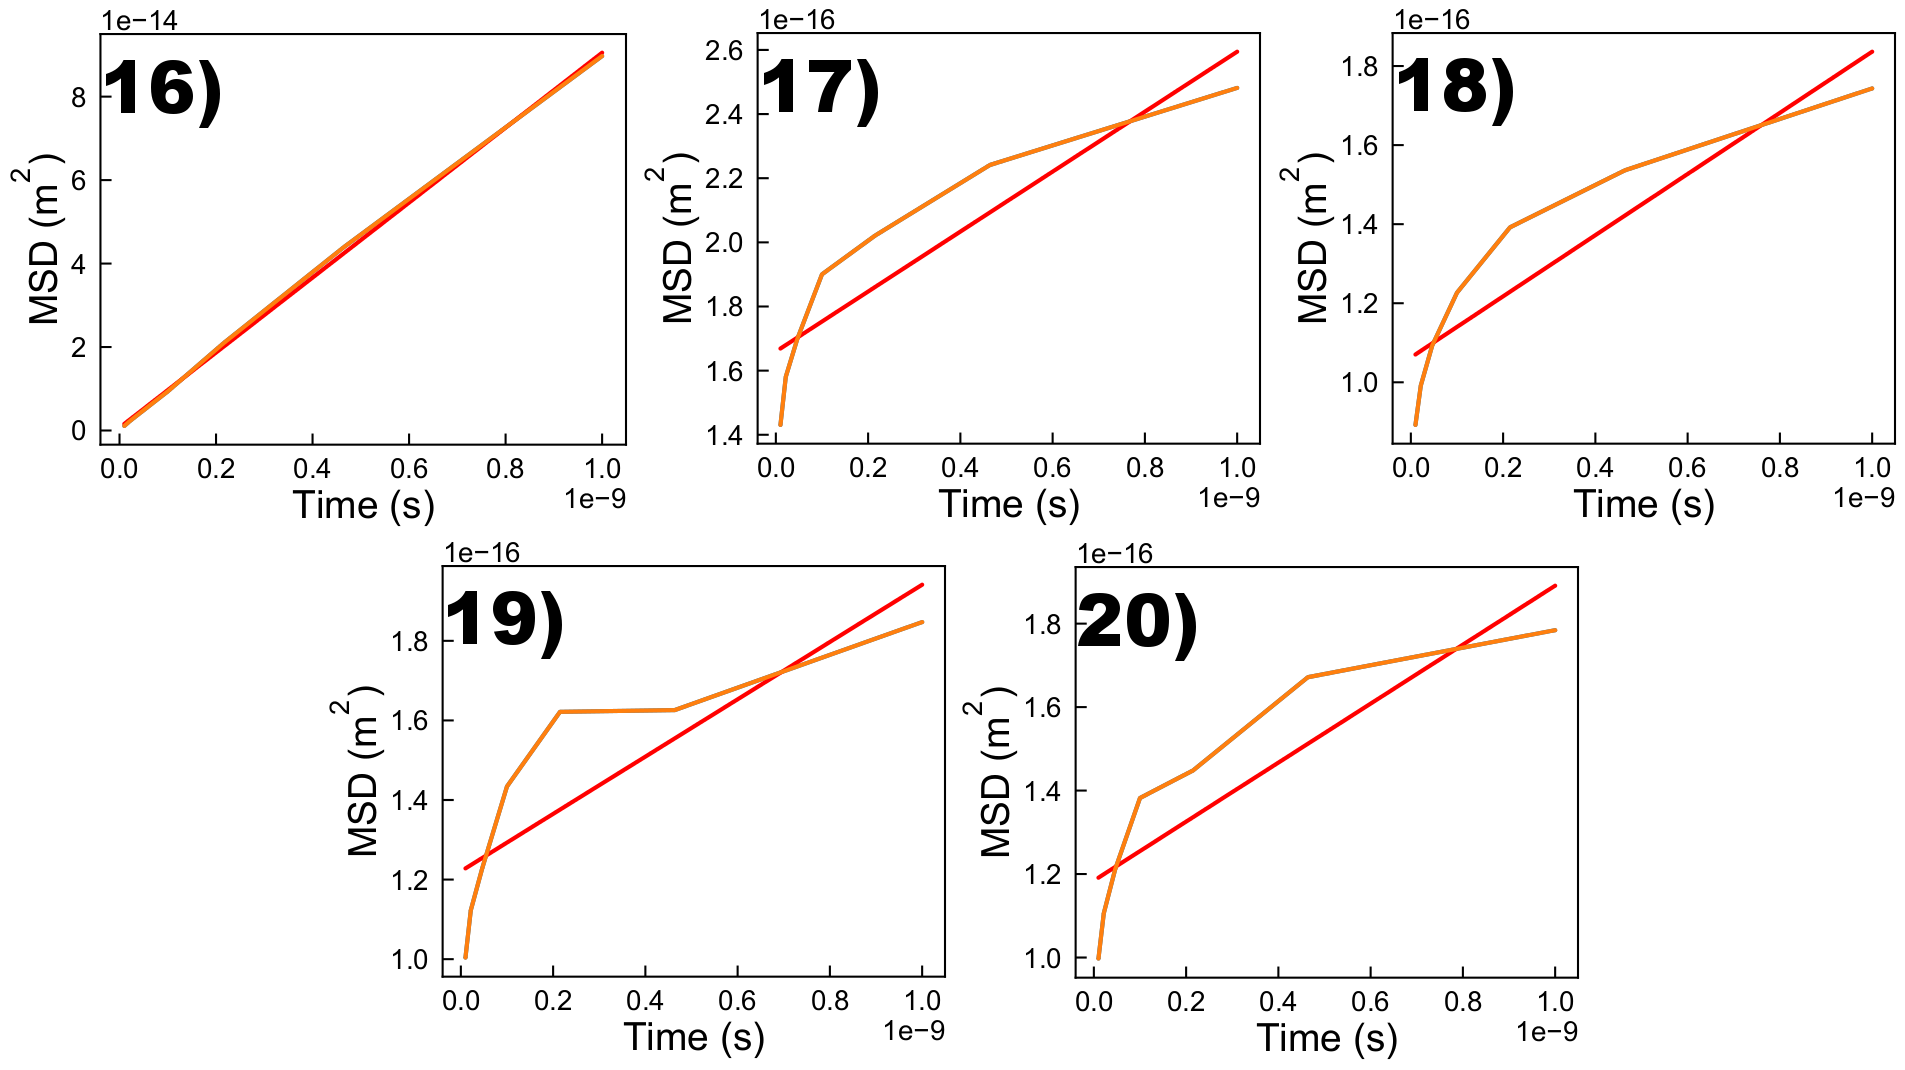
\includegraphics[width=\textwidth]{Figures/LinMSDHoleOrig.png}
    \caption{The linear mean squared displacement curves of the carriers within the morphologies \textbf{16} - \textbf{20}.}
	\label{fig:MSDOrig}
\end{figure}

\begin{figure}[h!]\centering
	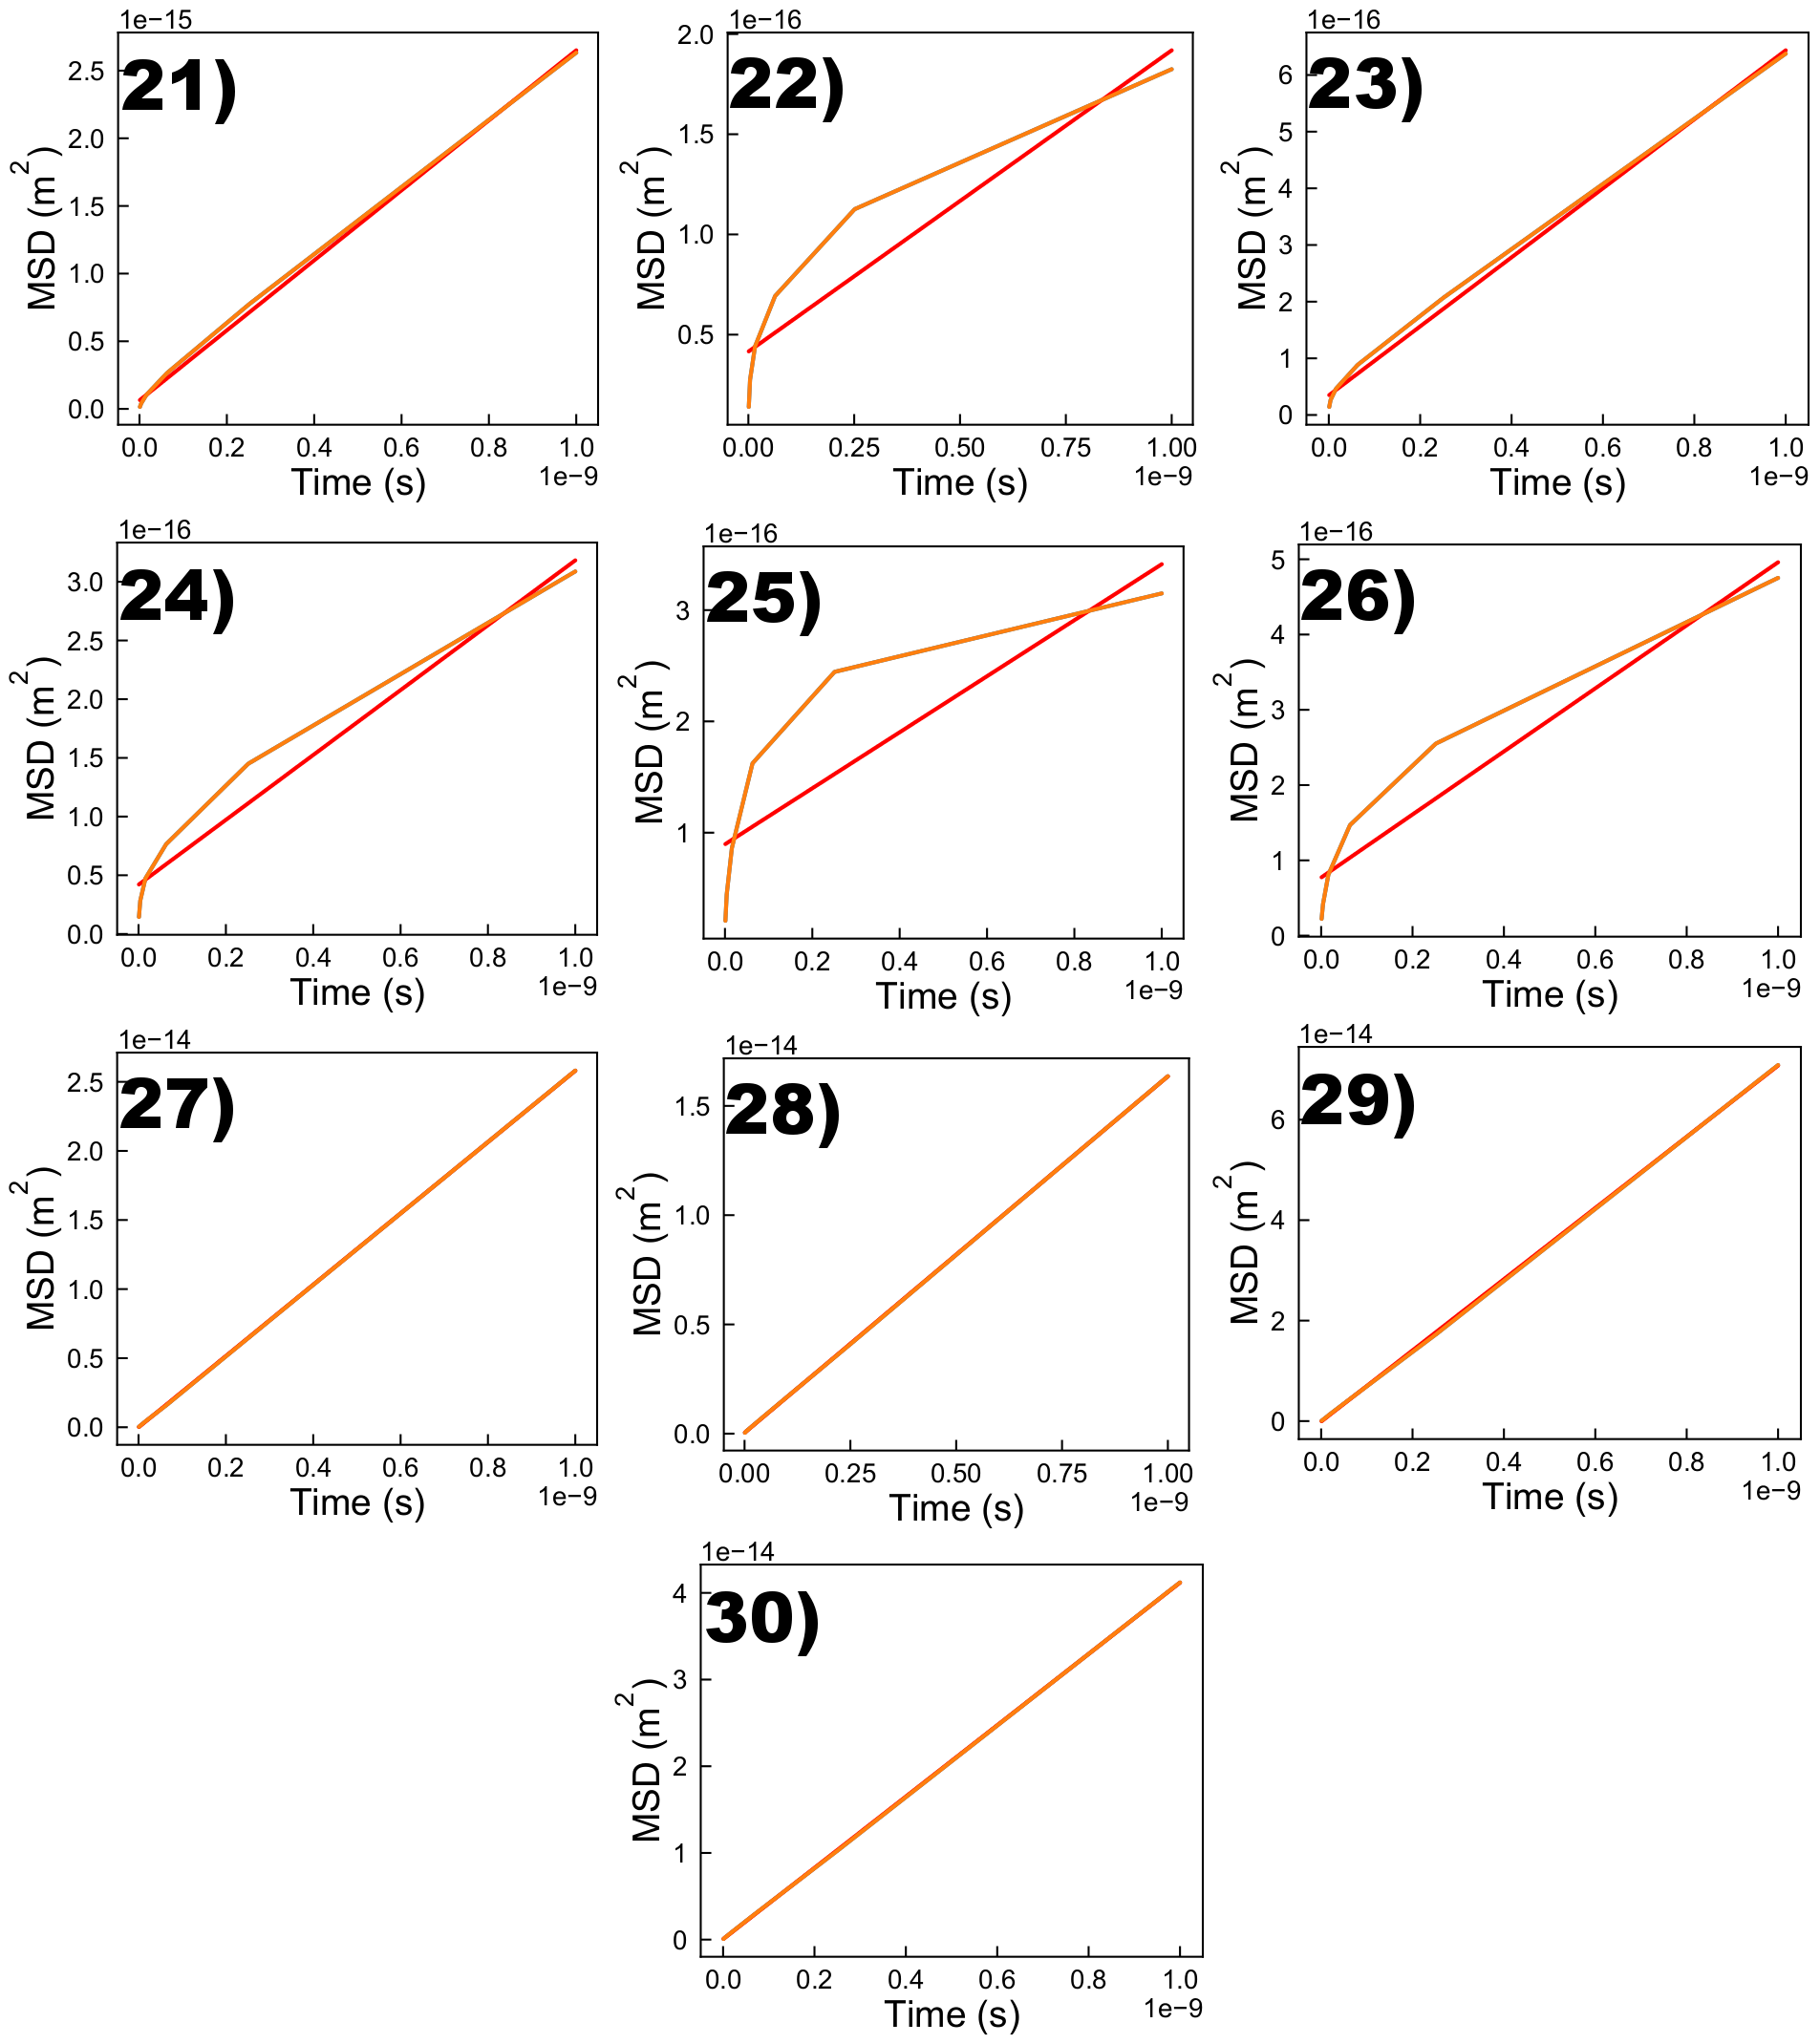
\includegraphics[width=\textwidth]{Figures/LinMSDHoleFrameOrig.png}
    \caption{The linear mean squared displacement curves of the carriers within the morphologies \textbf{21} - \textbf{30}.}
	\label{fig:MSDFrameOrig}
\end{figure}


\clearpage
\subsection{Hopping Rate Distributions}

\begin{figure}[h!]\centering
    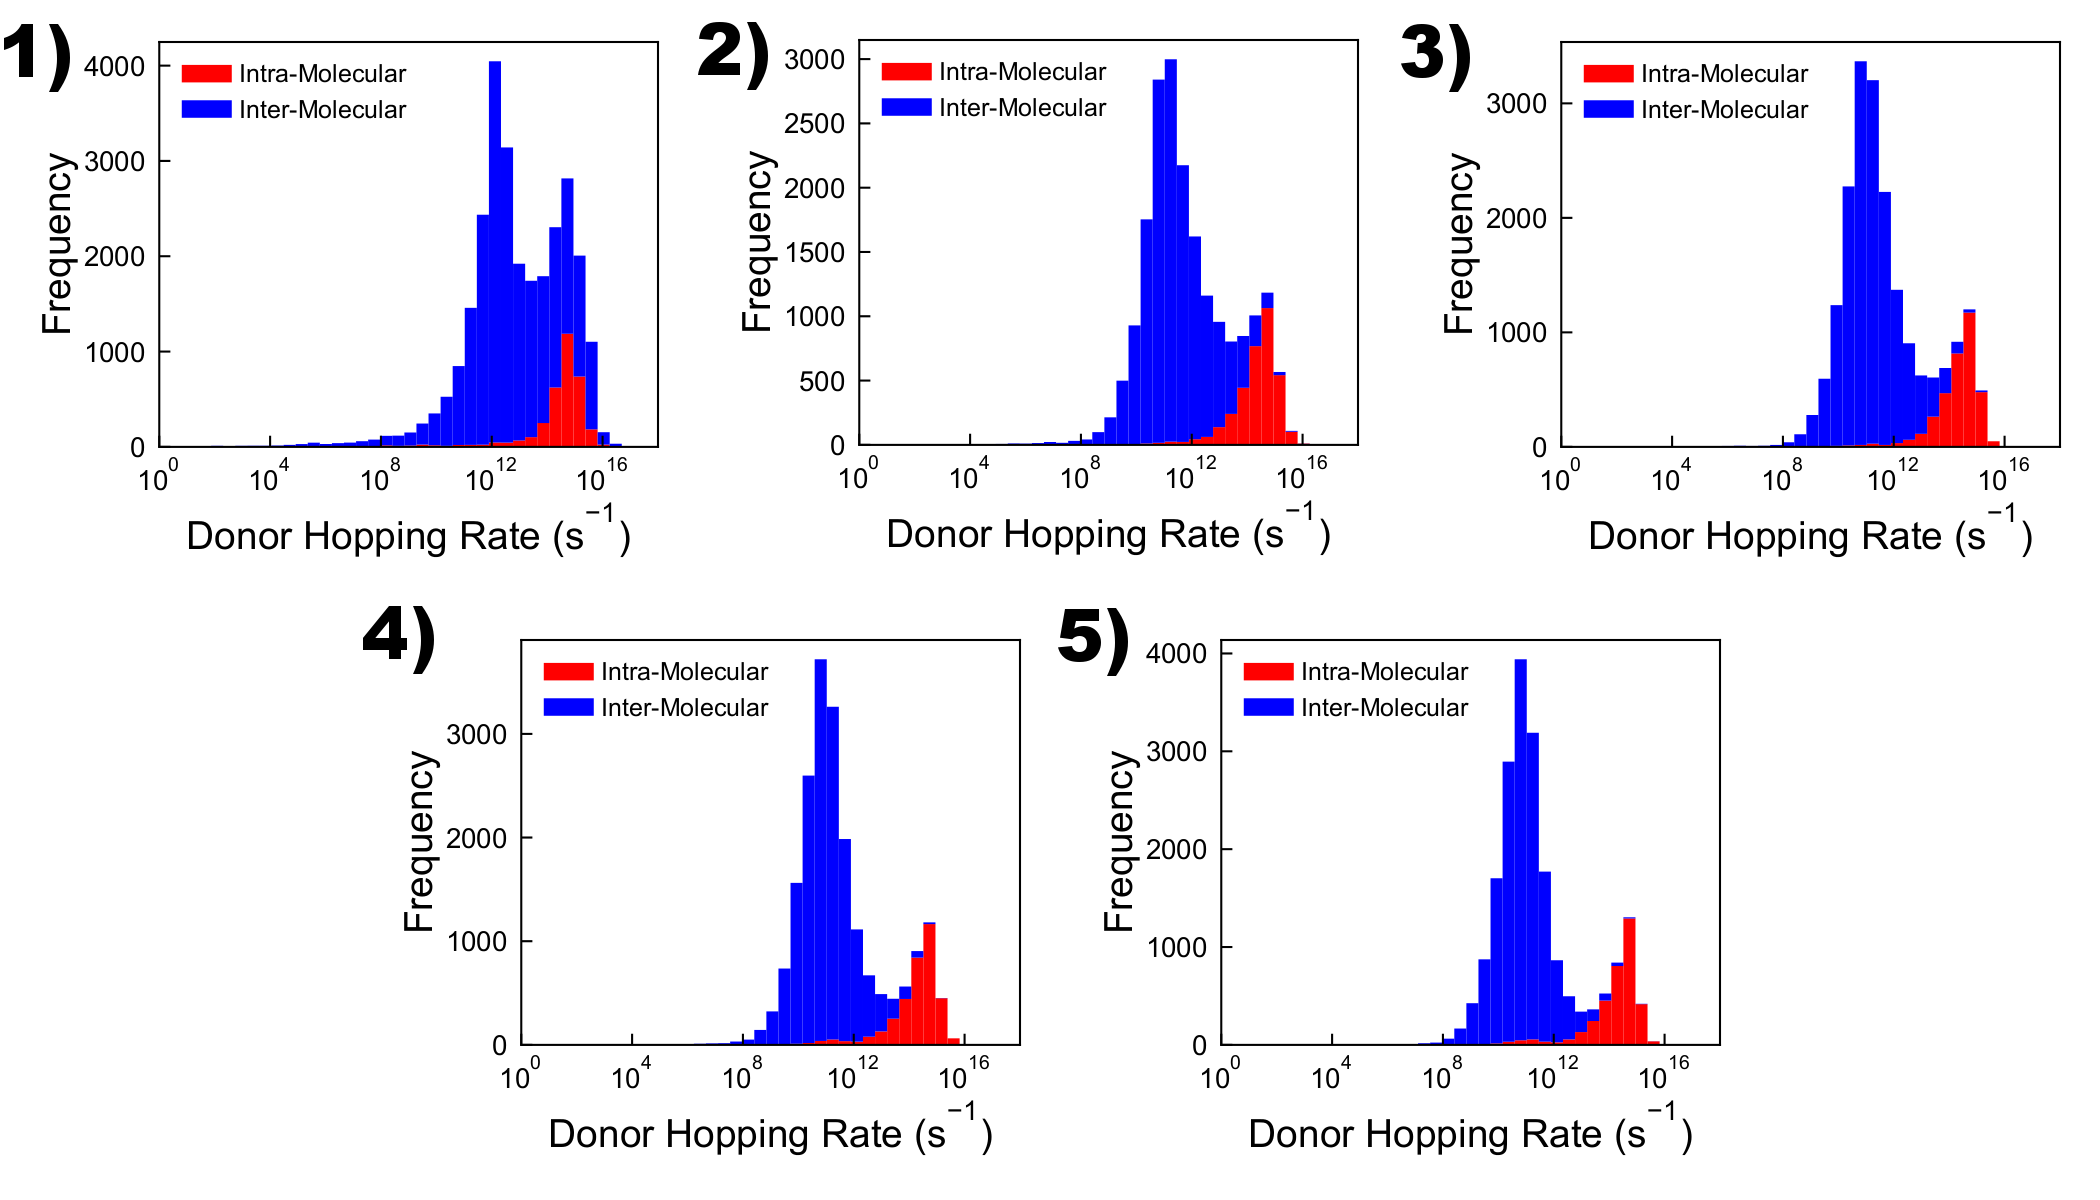
\includegraphics[width=\textwidth]{Figures/DonorHoppingRateMixed.png}
    \caption{The stacked hopping-rate distributions for intra- and inter-molecular hops executed by carriers within the morphologies \textbf{1} - \textbf{5}.}
	\label{fig:HoppingRateMixed}
\end{figure}

\begin{figure}[h!]\centering
    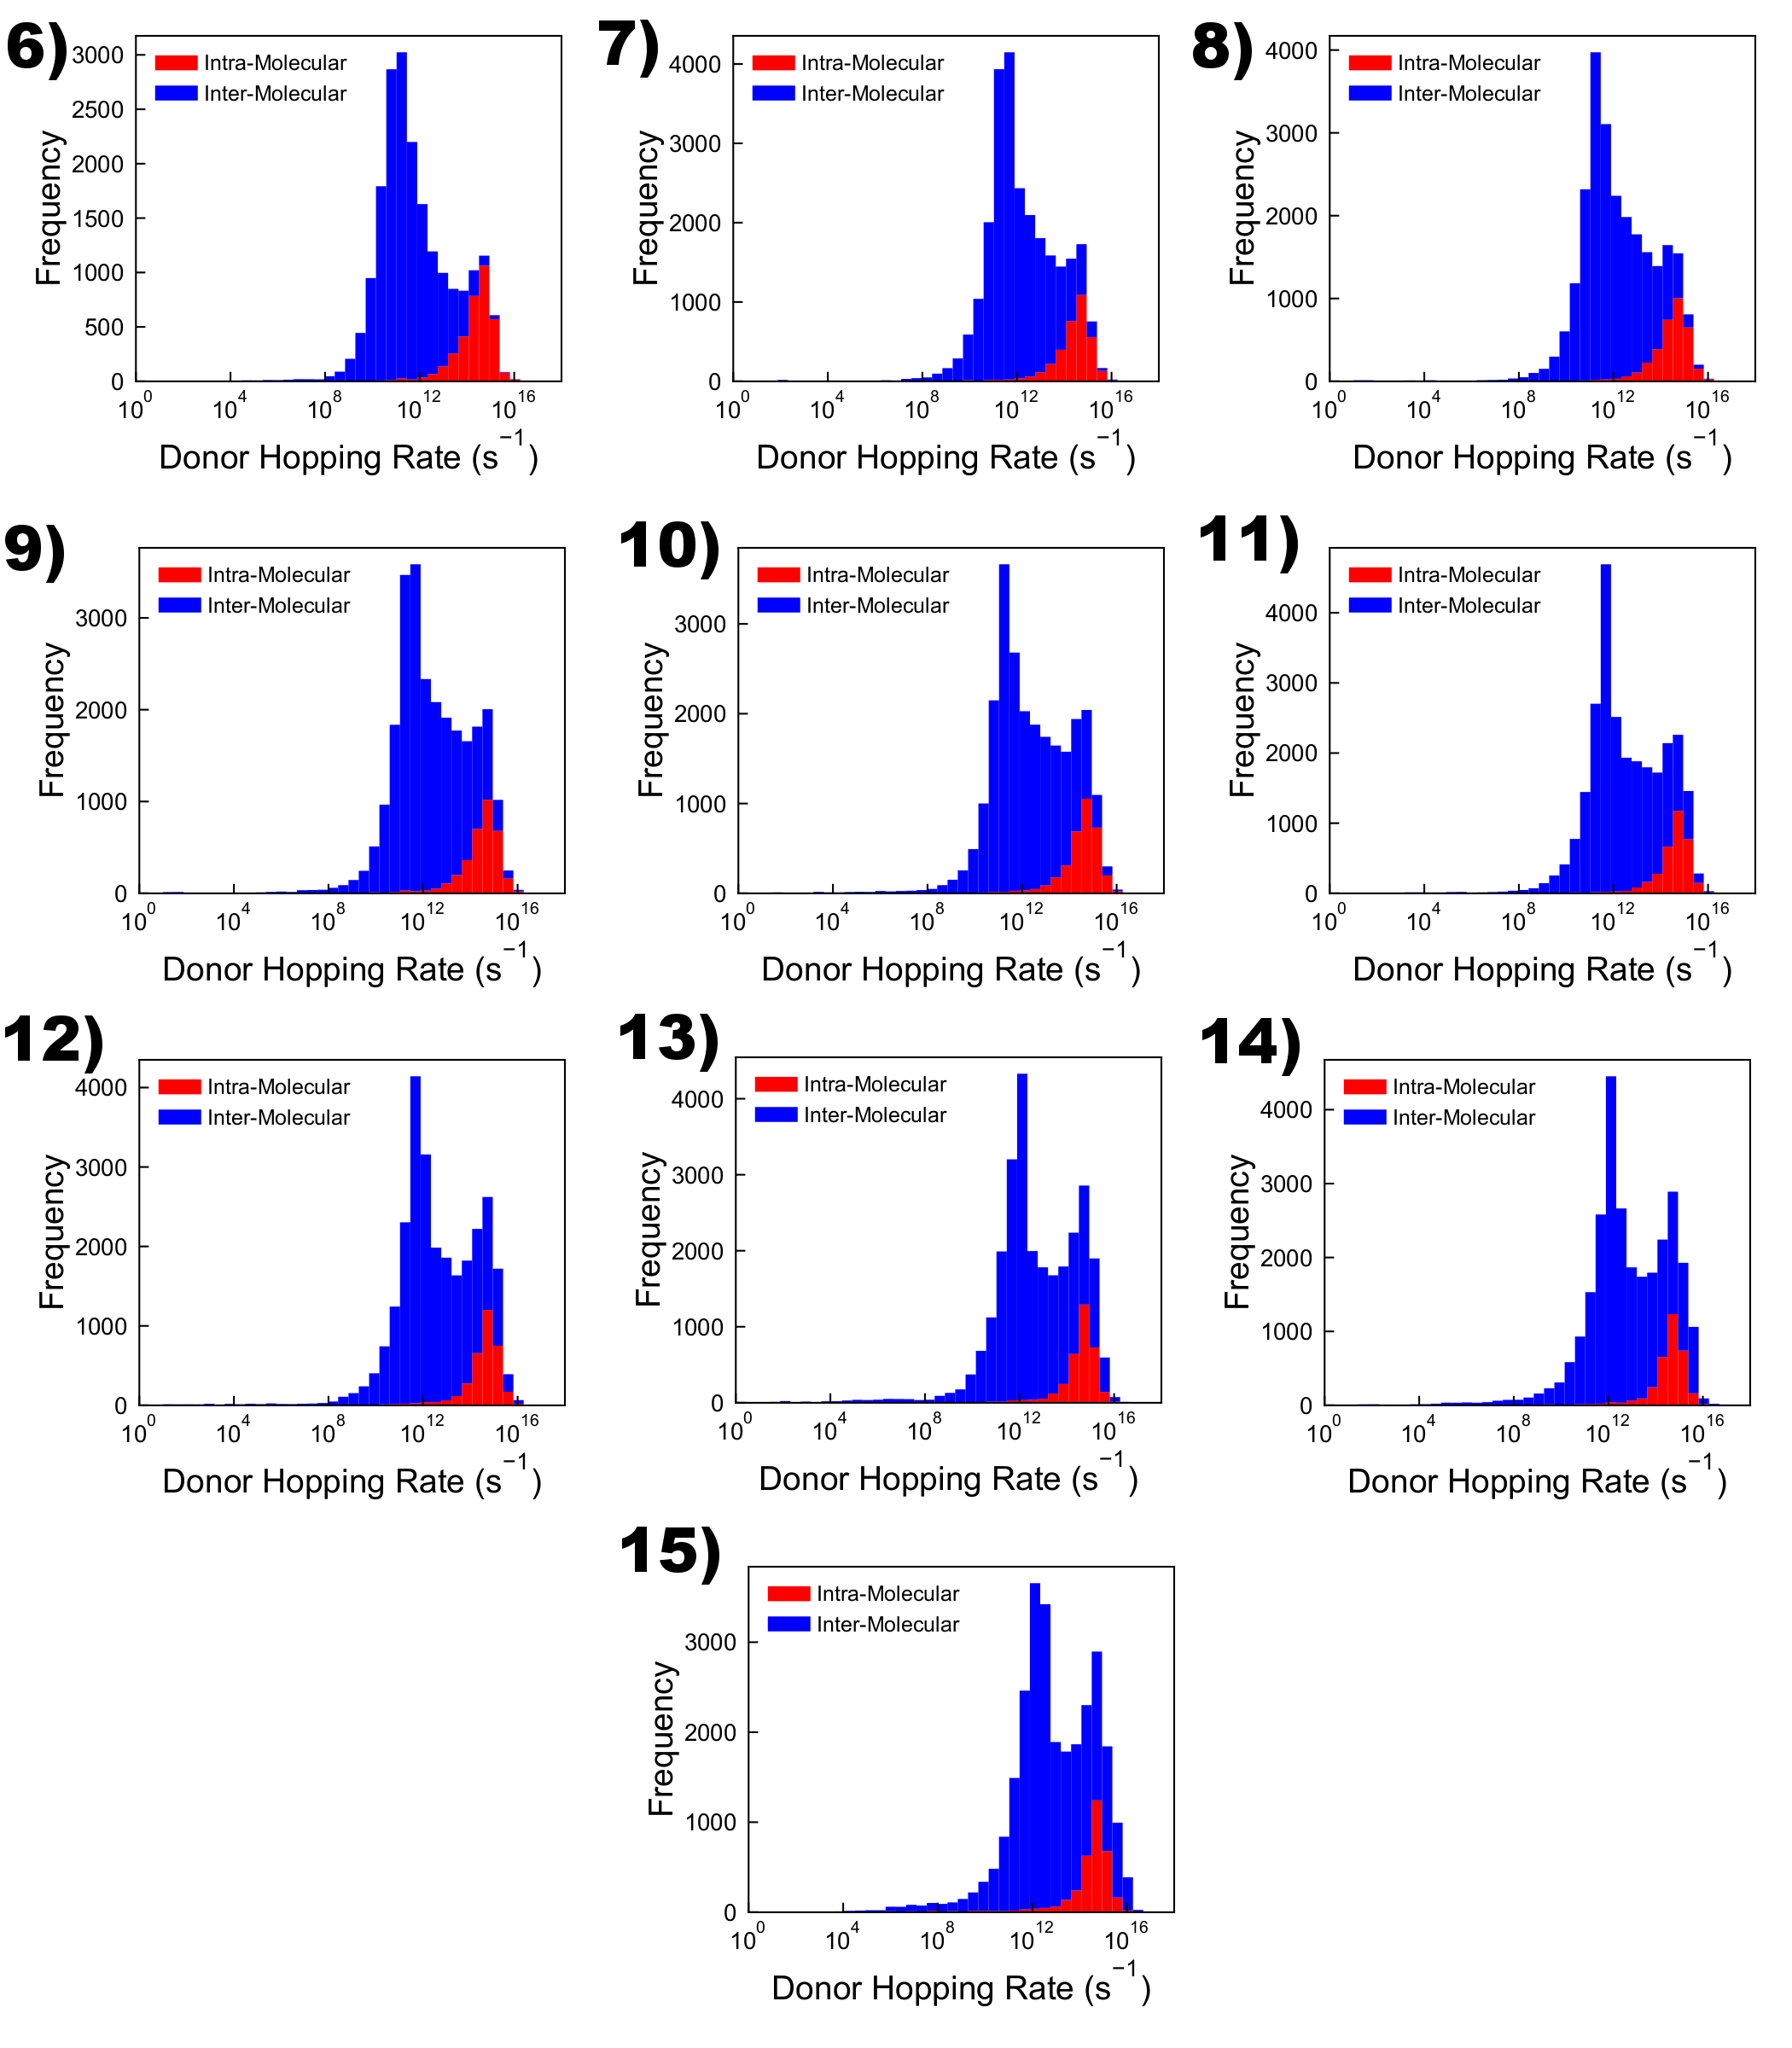
\includegraphics[width=\textwidth]{Figures/DonorHoppingRateMixedFrame.png}
    \caption{The stacked hopping-rate distributions for intra- and inter-molecular hops executed by carriers within the morphologies \textbf{6} - \textbf{15}.}
	\label{fig:HoppingRateMixedFrame}
\end{figure}

\begin{figure}[h!]\centering
    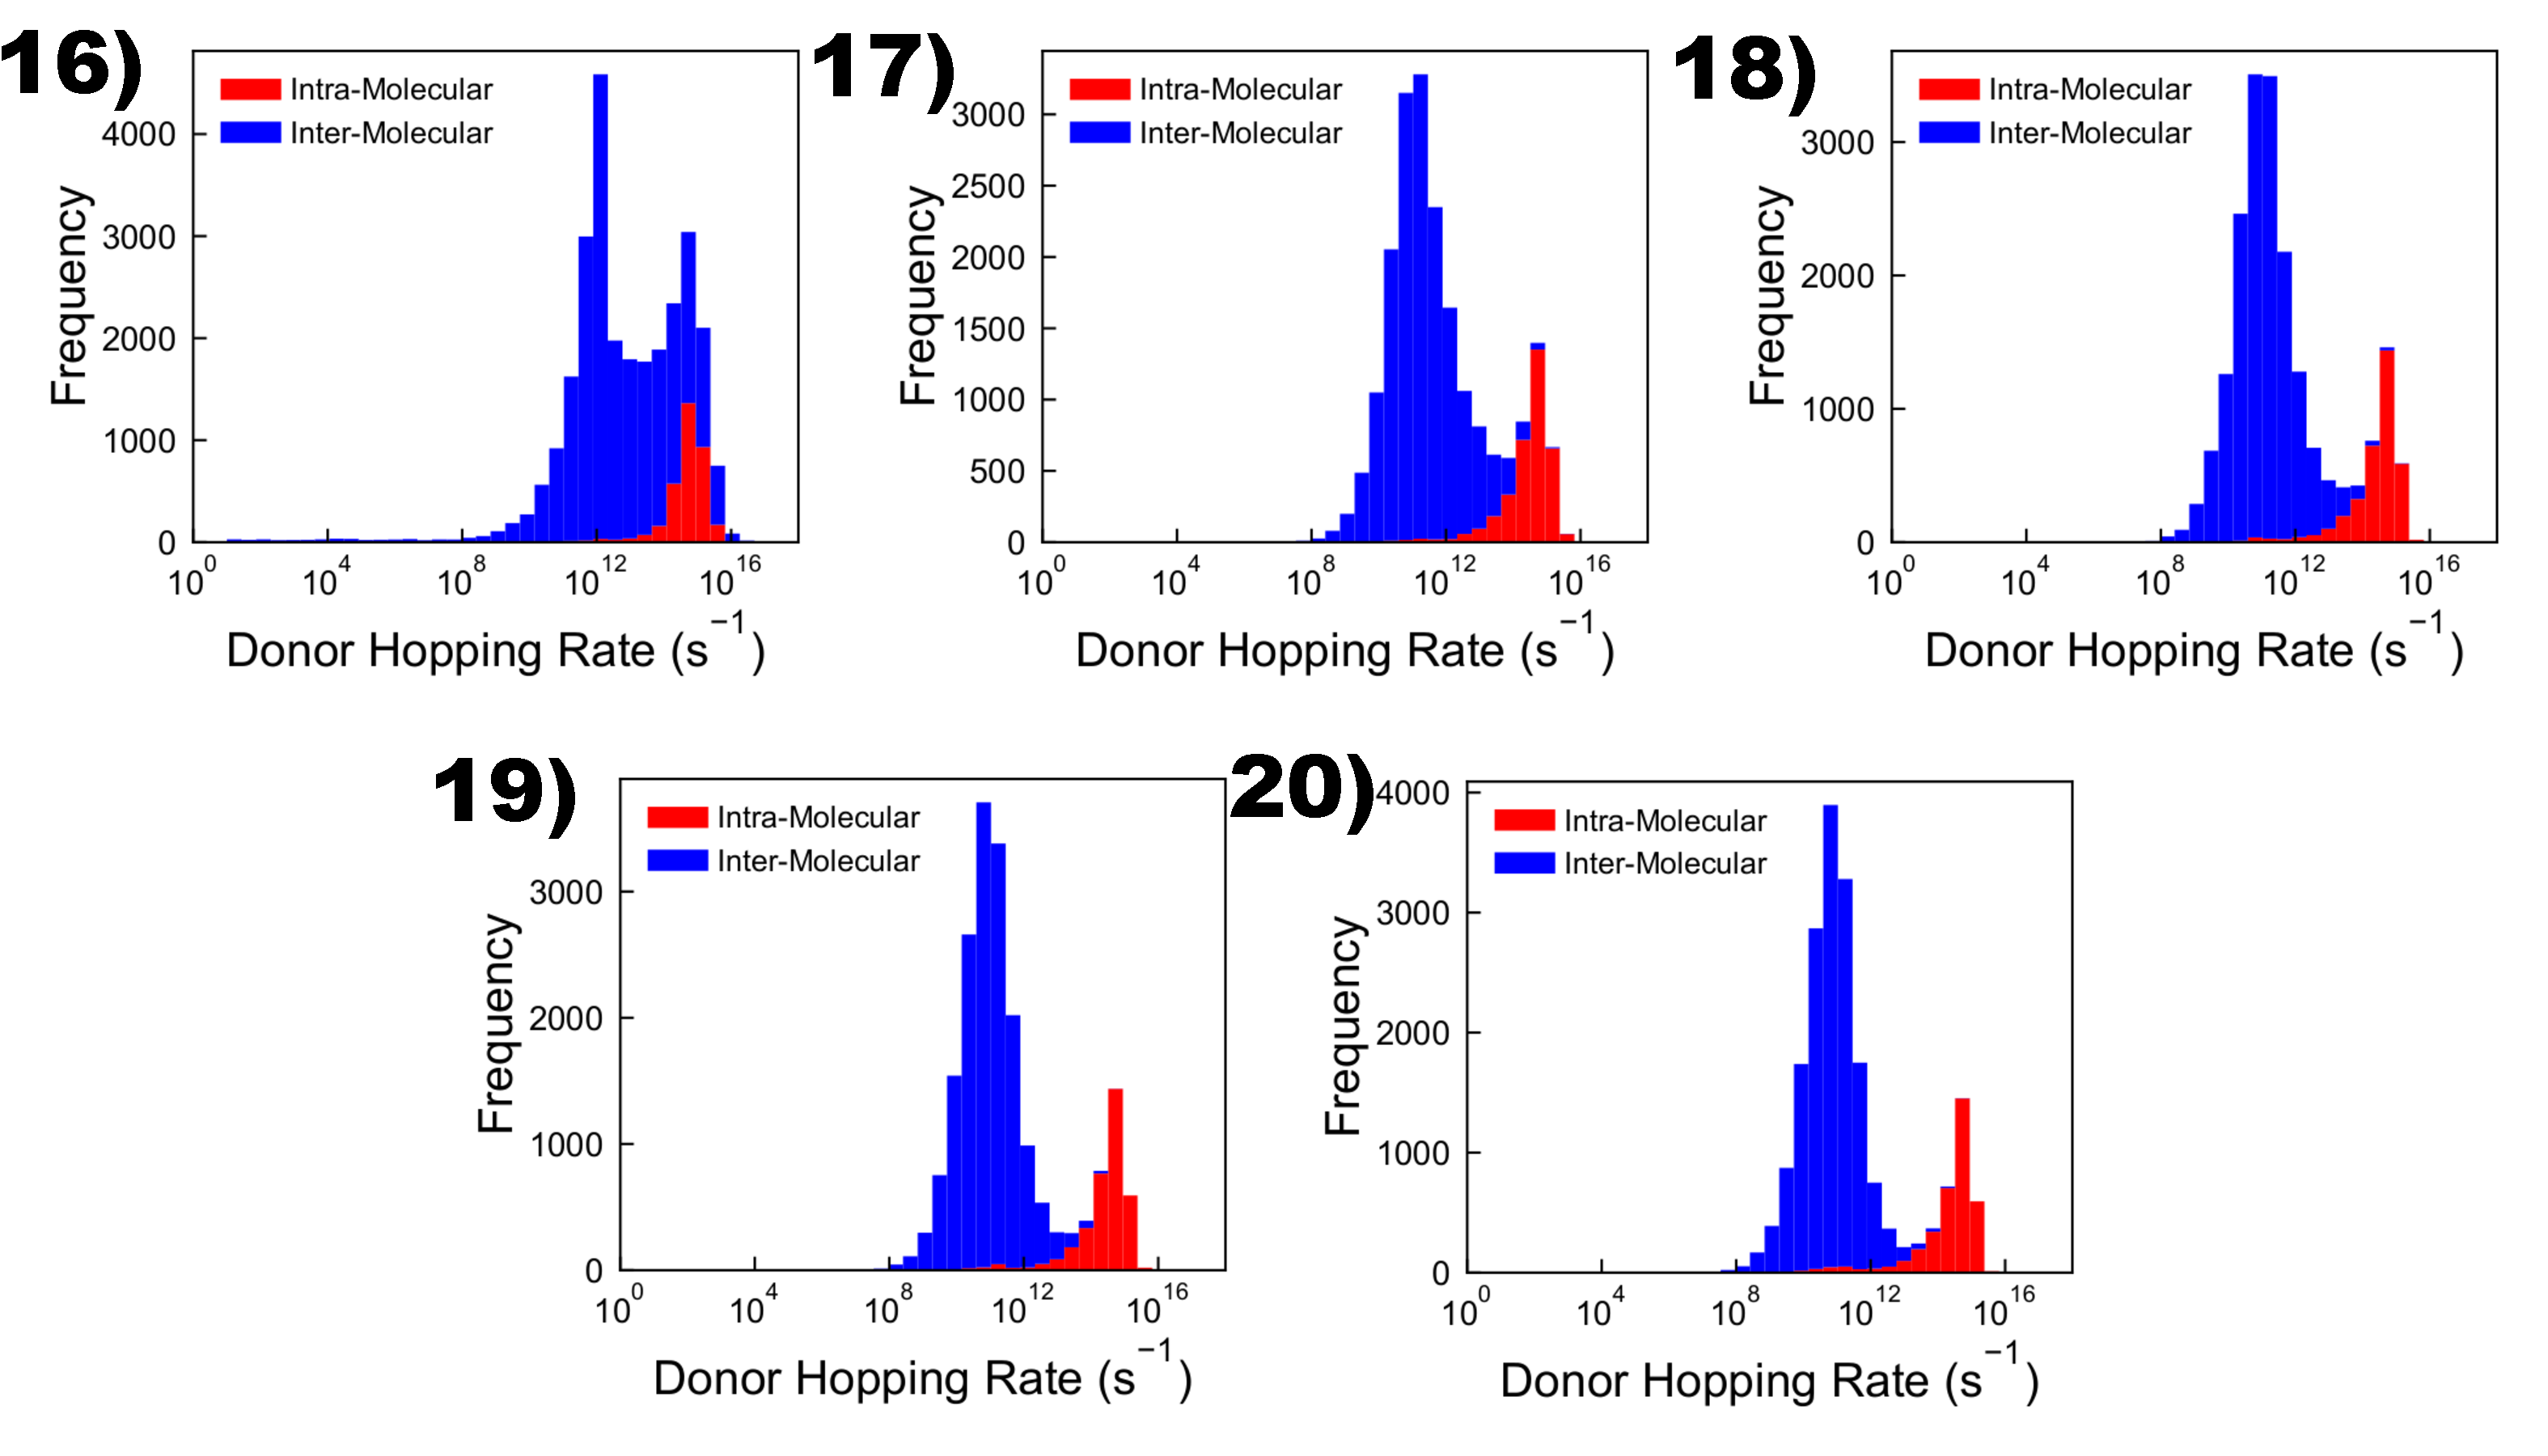
\includegraphics[width=\textwidth]{Figures/DonorHoppingRateMixedOrig.pdf}
    \caption{The stacked hopping-rate distributions for intra- and inter-molecular hops executed by carriers within the morphologies \textbf{16} - \textbf{20}.}
	\label{fig:HoppingRateMixedOrig}
\end{figure}

\begin{figure}[h!]\centering
    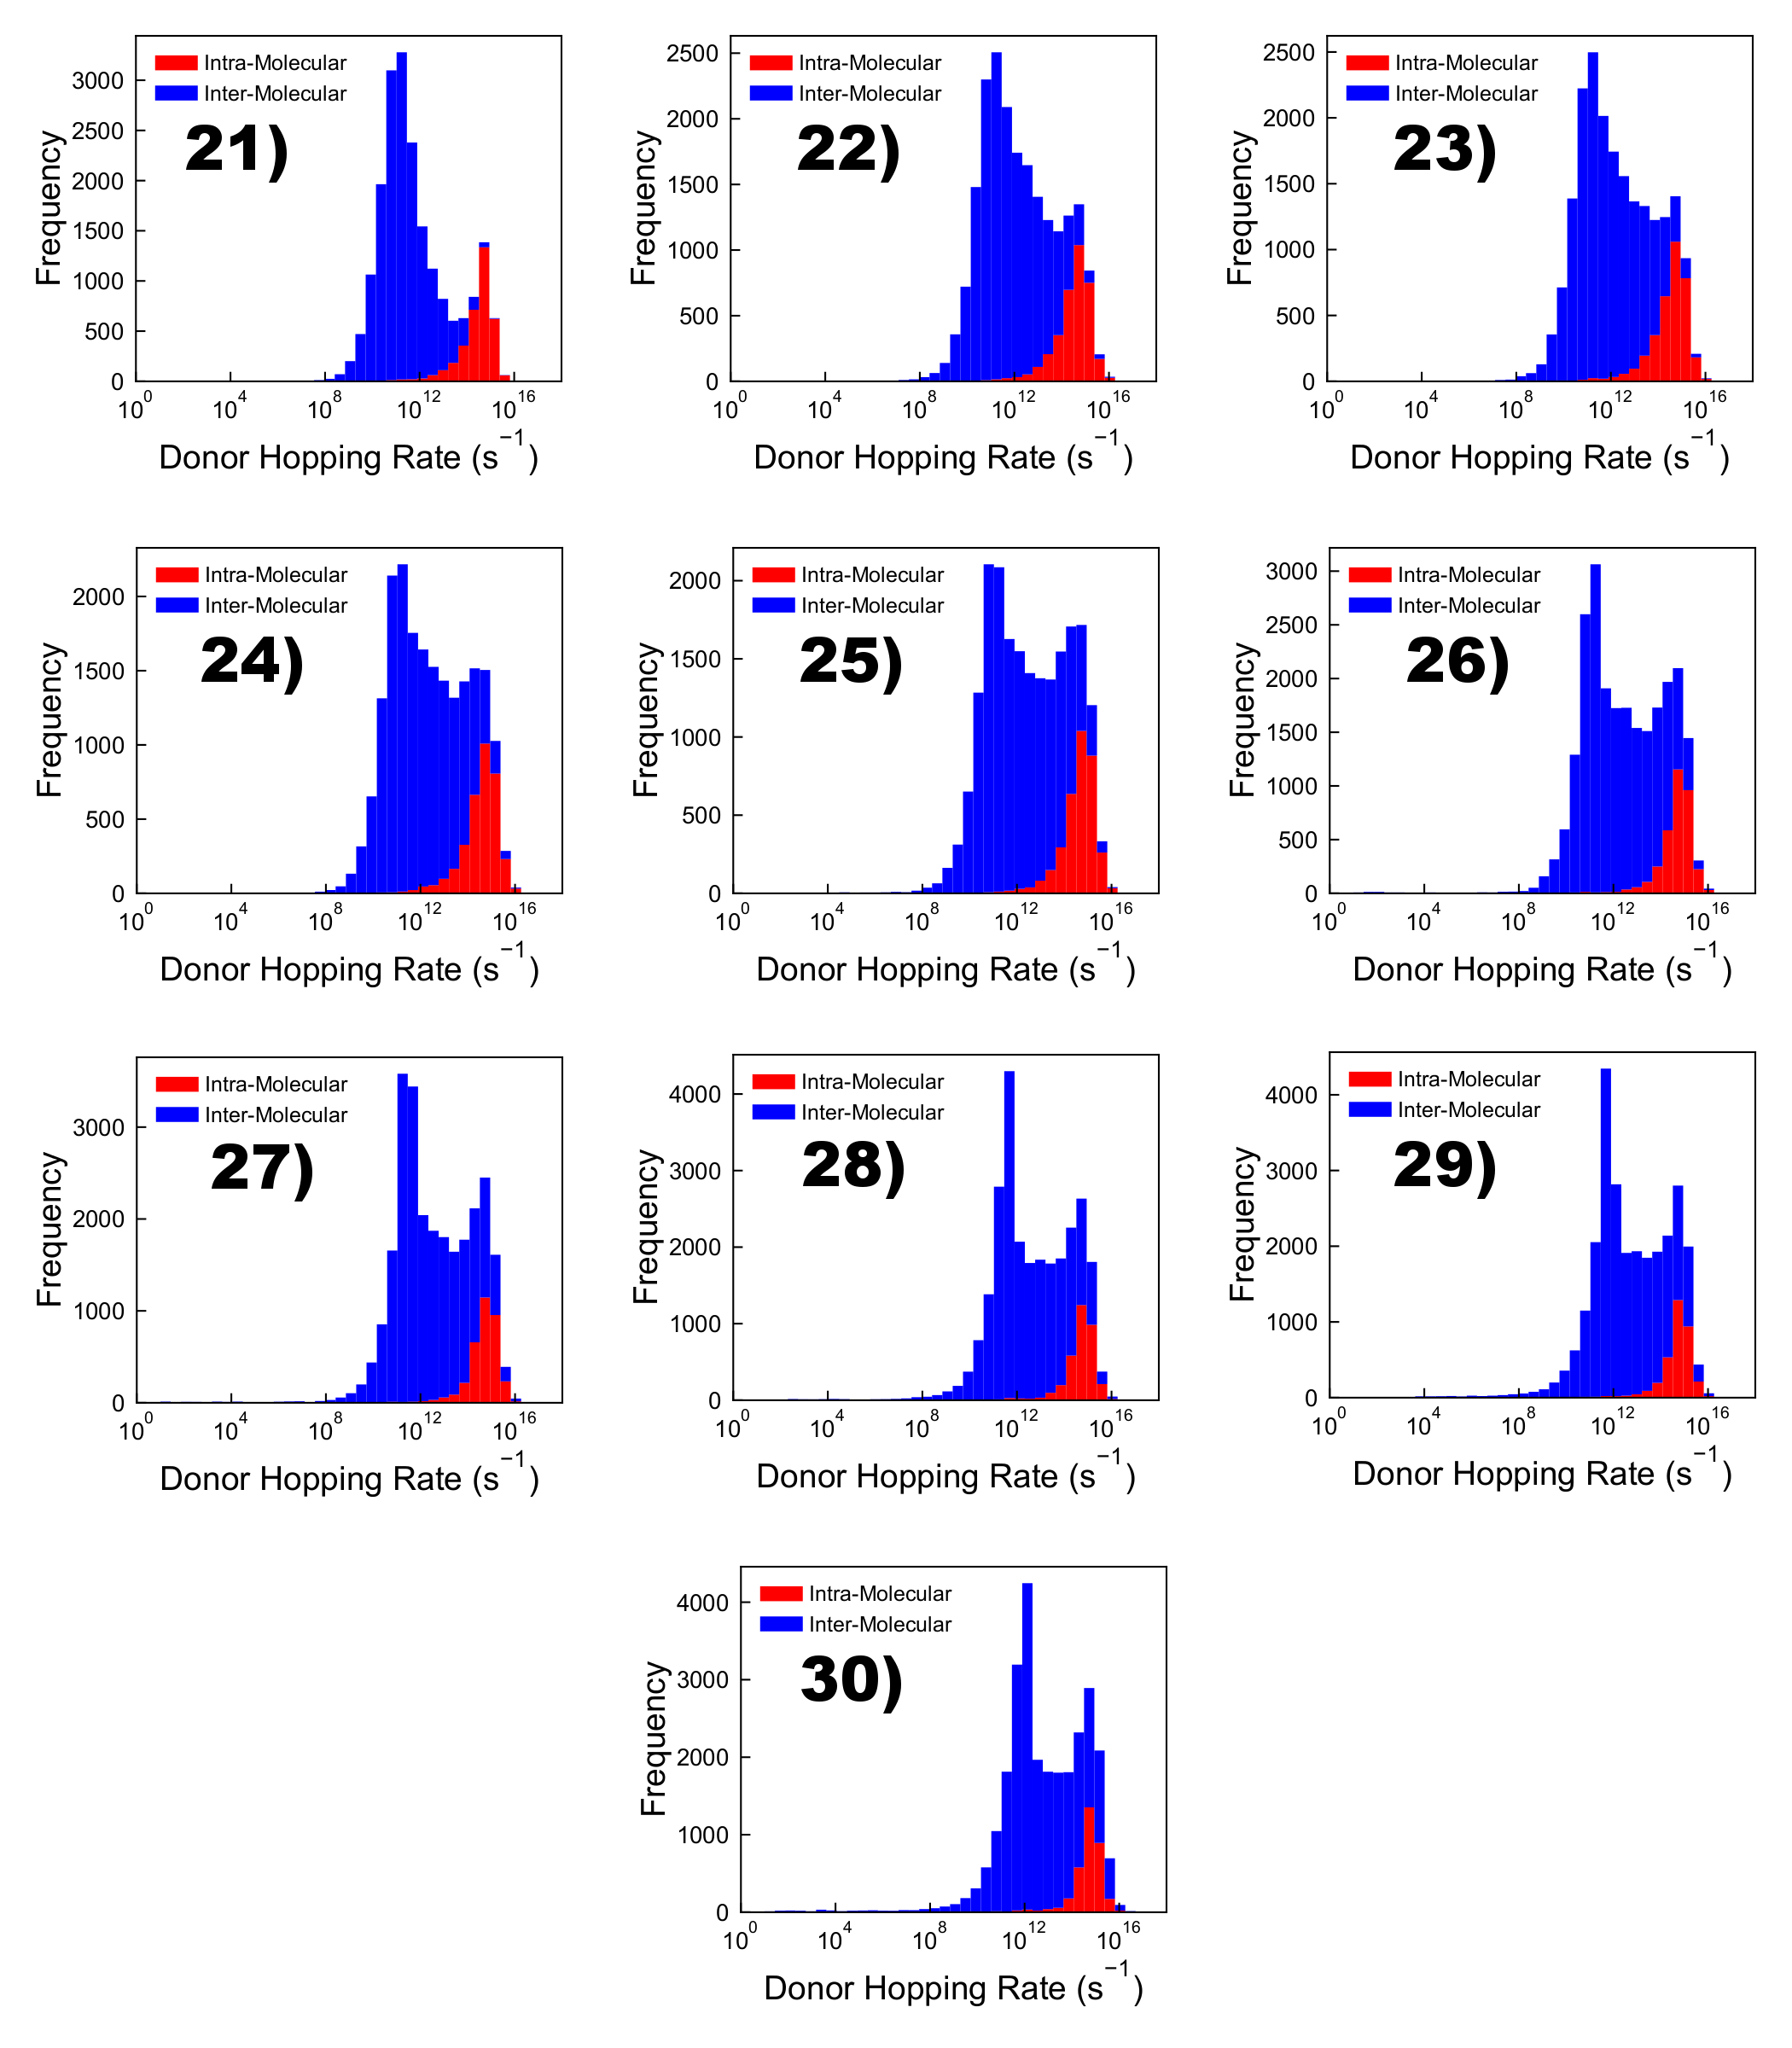
\includegraphics[width=\textwidth]{Figures/DonorHoppingRateMixedFrameOrig.png}
    \caption{The stacked hopping-rate distributions for intra- and inter-molecular hops executed by carriers within the morphologies \textbf{21} - \textbf{30}.}
	\label{fig:HoppingRateMixedFrameOrig}
\end{figure}

\clearpage


\bibliography{refs}
\bibliographystyle{unsrt}


\end{document}
